\documentclass[12pt,a5,twoside]{book}
\usepackage{blindtext}
\usepackage{geometry}
\usepackage[utf8]{inputenc}
\usepackage[spanish]{babel}
\usepackage{fancyhdr}
\usepackage{titlesec}
\usepackage{indentfirst}
\usepackage{lipsum}
\usepackage[numbers, super]{natbib} 
\usepackage[superscript,biblabel]{cite}
\usepackage{graphicx}
\usepackage[export]{adjustbox}
\usepackage{amsmath}
\usepackage{textcomp}
\usepackage{subfigure}
\usepackage[stable]{footmisc}

\renewcommand{\thefootnote}{\alph{footnote}}
\pagestyle{headings}
\rfoot{\thepage}

\begin{document}

\chapter{Imágenes de resonancia magnética funcional}

Aquí hay algunos conceptos muy básicos sobre el origen de la señal fMRI y cómo ésta es analizada. Este capítulo no pretende ser una revisión completa acerca del tema. Para mayores detalles, el lector deberá referirse a las numerosas y valiosas revisiones acerca del tema, así como docenas de sitios web con tutoriales y audio-visuales que brindan ayuda para entender cómo está técnica trabaja.\footnote{http://www.psy.vanderbilt.edu/tonglab/sonia/Personal/fMRI\_Basics.html\\ http://afni.nimh.nih.gov/pub/dist/edu/lastest/afni01\_intro/FMRI\_basics.pdf\\http://neuroeconomics\-summerschool.standford.edu/pdf/ODoherty\_fMRI.pdf}

Si usted encuentra errores, imprecisiones o errores tipográficos, por favor, contacte al autor para que sean corregidos.

\section{Contraste de Oxigenación Nivel Dependiente (OND)}

En las imágenes obtenidas por resonancia magnética, toda la señal es producida por la resonancia de los momentos magnéticos inherentes a los espines de los protones dentro de las moléculas de agua (sí, eso se come). Para protones individuales, la magnitud de esta señal es despreciable pero, afortunadamente, nuestro cuerpo está compuesto por aproximadamente 70\% de agua, por lo tanto, en promedio, hay mucha señal. Además, en virtud de estar dentro de un campo magnético muy grande (por ejemplo, 1.5 o 3 Tesla), estos momentos magnéticos se alinean con el campo magnético principal, dándonos la oportunidad de hacer sus resonancias coherentes. Sin entrar en detalles, estos espines son invisibles a la bobina de recepción mientras están alineados al campo magnético principal, pero si los alteramos con una radiofrecuencia muy específica (generalmente en el rango de FM), entonces, podemos colocarlos ortogonalmente al campo magnético principal, en torno al cual precesarán (girarán alrededor de él) produciendo una frecuencia resonante que la antena puede registrar. Si están todos precesando a la misma frecuencia y, muy importante, con la misma fase, el vector resultante de la suma de cada espín será de gran tamaño y nuestra señal neta. Por lo tanto, aumentará. Por otro lado, aunque estos espines estén precesando a la misma frecuencia, pueden estarlo haciendo a distinta fase, en cuyo caso, nuestra señal neta será igual a cero. Así como sucedería en una carrera de los 400 metros planos, todos los corredores inician a correr juntos, pero luego de un tiempo, notamos que algunos corredores son más rápidos que otros y esto provoca que el grupo de corredores se disperse. Lo mismo sucede con los espines, al iniciar todos tienen la misma fase, sin embargo, debido a que algunos espines están precesando ligeramente más rápido que otros, un tiempo después el ensamble pierde la fase. Pero, ¿cuál es la causa de las diferencias de velocidad en la precesión de los espines? La respuesta es simple: el campo magnético con el cual interactúan. Esto sucede en una relación linear de acuerdo a la ecuación de Larmour:

\begin{equation} 
\omega = \gamma \it{B_{0}} 
\end{equation} 

dónde \(\omega\) es la frecuencia de precesión del espín, \(B_{0}\) es el campo magnético que experimenta el espín en cuestión y \(\gamma\) es el radio giromagnético del Hidrógeno (42.5 MHz/T). Este fenómeno es la base de todos los tipos de codificación en la RM, desde la selección de cortes, la codificación espacial, hasta la creación de contrastes, como OND o imágenes pesadas a difusión (Capítulo 2).

Muchos factores pueden alterar el campo magnético experimentado por los protones. Por ejemplo, \(B_{0}\) se puede modificar explícitamente sumando o restando un campo secundario creando un gradiente lineal, que es el principal medio de codificación espacial para obtener imágenes 2D o incluso 3D. Sin embargo, las modificaciones de \(B_{0}\) pueden ocurrir a escala microscópica, como sucede en presencia de metales que se acumulan en ciertos tejidos del cerebro, como son los ganglios basales. Ahora, recordemos qué en el corazón de la molécula que transporta oxígeno, la hemoglobina, encontramos Hierro (Fe). Como su nombre indica, Fe es altamente ferromagnético, por lo que no es extraño considerar su interacción con \(B_{0}\) y, por tanto, modificar \(\omega\). Dos cosas son particularmente interesantes acerca del Fe contenido en la hemoglobina: primero, fluye, no es estacionario (a menos que se trate de un coágulo); Y en segundo lugar, interactúa de manera diferente con \(B_{0}\) dependiendo si la molécula lleva Oxígeno o no. La hemoglobina desoxigenada (dHb) es paramagnética y crea gradientes magnéticos microscópicos dentro y alrededor de los vasos sanguíneos, desfasando los espines y reduciendo la señal recibida. Este fenómeno fue descubierto por primera vez por Ogawa en 1990 \citep{OgawaS1990}, dando origen a todo el campo de la RMf que floreció en la primera década de los años 2000's y se está reinventando en el presente. En otras palabras, dHb ocasiona que perdamos la señal constantemente. Sin embargo, cuando un área particular de corteza está involucrado en una tarea particular, el flujo sanguíneo se incrementa focalmente, incluso superando la tasa metabólica cerebral de oxígeno.
Esto a su vez conduce a un {\it exceso} de Hb (Hbo) oxigenada con respecto a Hbd, y la pérdida previa de señal disminuye. En efecto, si comparamos la cantidad de señal durante un período activo que induce un aumento de Hbo veremos una {\it ganancia de señal} con respecto al período inactivo. Este efecto es más notable en las imágenes en las que el contraste de T2* se maximiza, generalmente realizado usando ecos de gradiente (aunque este es un concepto crucial, no entraremos en la física detrás de él). 

La respuesta vascular al aumento de la actividad neural no es inmediata, sino relativamente lenta, tanto para iniciar como para regresar a la línea de base. Esto se llama la función de respuesta hemodinámica (FRH) y, aunque su forma es diferente en distintas porciones del cerebro, una FRH ``canónica'' se utiliza generalmente en el análisis IRMf a través del volumen cerebral y puede verse en la Figura 1.1. 

\begin{figure}
	\centering
	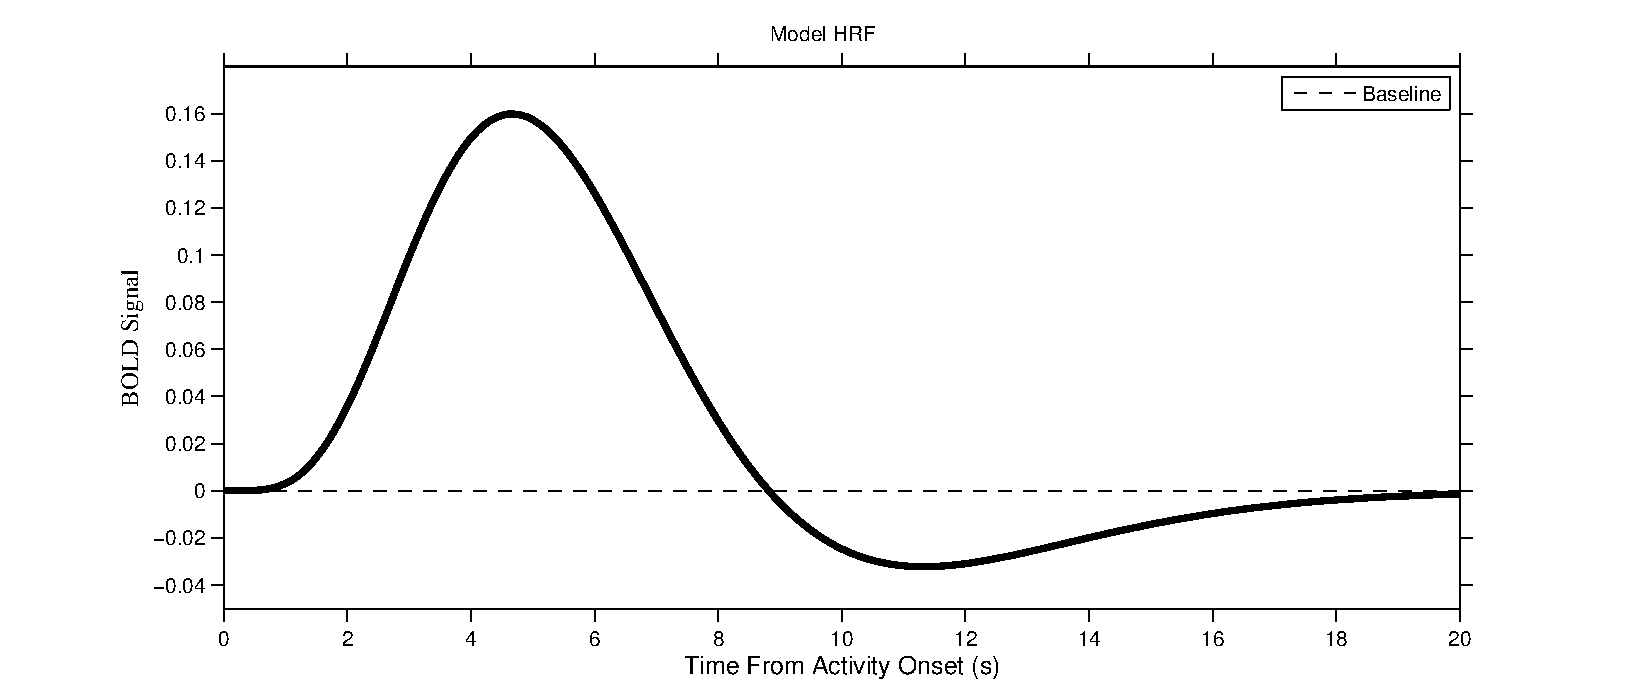
\includegraphics [scale=0.6,center] {HRF.eps}
    \caption{\textbf{Función de respuesta hemodinámica canónica (FRH) a un estímulo instantáneo centrado en 0 segundos.} El flujo sanguíneo aumenta dos segundos después del estímulo y alcanza un pico en torno a los 4 segundos. Hay un subestimado post-estímulo entre 8 y 20 segundos, después de lo cual la señal (unidades arbitrarias) regresa a la línea de base. Este FRH es modelado por la suma de dos distribuciones gamma (aprender a hacer su propio diagrama FRH en http://thelevermahine.wordpress.com/tag/hemodynami-response-funtion)}
    \label{F:HRF}
\end{figure}

El acoplamiento neuro-vascular necesario para producir la FCH todavía se debate. Sin embargo, los astrocitos parecen jugar un papel crucial en su generación, ya que poseen un proceso vascular que interactúa con las paredes de los vasos produciendo la vasodilatación necesaria y el aumento del flujo. Los astrocitos absorben glutamato y lo metabolizan a glutamina, en un proceso que es dependiente de ATP. La hidrólisis del ATP aumenta en última instancia la concentración intracelular de Ca, que a su vez activa una vía de señalización que da lugar a la liberación de prostaglandinas en el proceso vascular del astrocito que modula la formación de AMPc en la musculatura de la pared vascular, dilatado \citep{KoehlerRC2009}.

Una propiedad interesante de la FRH es su linealidad. Es decir, varios FRHs se suman para producir una sola respuesta (Figura 1.2). Si los estímulos o actividades están muy juntos en el tiempo, los FRHs se agruparán en una sola función de respuesta que será una versión modificada de un bloque de actividad. Podemos saber de antemano cuál será la forma de la FRH si conocemos los momentos de estimulación/actividad. Para el caso de un solo estímulo corto, sabemos que el FRH resultante es simplemente el FRH canónico, pero en el caso de conjuntos de estímulos que están muy juntos en tiempo o bloques de estimulación, el FRH resultante puede estimarse convolucionando el tiempo vector de estímulos con el FRH canónico. Los bloques resultantes o los FRH individuales se pueden ver en la Figura 1.3.

Podemos ver que hay dos maneras muy básicas de crear un paradigma de estimulación a lo largo de una sesión de IRMf: diseño de bloques o eventos. Ambos son esencialmente iguales y se procesan de maneras análogas, la principal diferencia es que en los diseños de bloques el estímulo o actividad es continuo durante un período de tiempo (generalmente 10-30 segundos), mientras que en diseños relacionados con eventos el estímulo/actividad está disperso a lo largo de la sesión de forma ordenada o al azar, dependiendo del experimento.

\section{Experimentos de IRMf}

El enfoque general para encontrar las áreas del cerebro que se activan durante una tarea dada es comparar la señal BOLD de cada voxel (elemento de volumen, un píxel en la jerga 3D) durante la tarea en comparación con la obtenida durante el reposo, o una diferente (control) tarea. Para hacer este análisis voxel por voxel, debemos obtener varias secciones del cerebro con resolución espacial y temporal decente. La resolución espacial oscila entre 4 mm y 1 mm en escáneres clínicos, pero puede ser mucho mayor en los escáneres de animales. La resolución temporal suele gravitar alrededor de 2-3 segundos, que es el tiempo necesario para obtener suficientes rebanadas para cubrir todo el cerebro usando imágenes ecoplanares en escáneres convencionales. Sin embargo, las técnicas recientes de adquisición de imágenes permiten una cobertura cerebral completa con resolución temporal inferior a un segundo \citep{Candes_2006}. El sujeto recibe instrucciones para realizar la tarea o sobre la naturaleza del paradigma de estimulación y, mientras está acostado boca arriba y todavía en el escáner, se le pide que realice la tarea o se estimule a través de algún aparato compatible con IRM (auriculares, proyector de pantalla, etc). El paradigma de la estimulación puede durar entre 3-4 minutos, sin embargo puede ser más largo si los sujetospuede permanecen interesados en la tarea sin moverse demasiado. En la práctica, paradigmas de más de 15 minutos tienden a inducir aburrimiento e pérdida de atención. Las tareas o estímulos se pueden realizar o presentar como bloques o como eventos aislados (Figura 1.3), dependiendo de la naturaleza del experimento \citep{Amaro_2006}. A modo de ejemplo, consideremos una tarea con un dedo en un diseño de bloque, con 30 segundos de actividad seguido de 30 segundos de descanso. Una alternancia de actividad-descanso se llama una ``época'', y nuestro experimento tiene 5 épocas, para un total de 5 minutos (Figura 1.4).

\begin{figure}
	\centering
    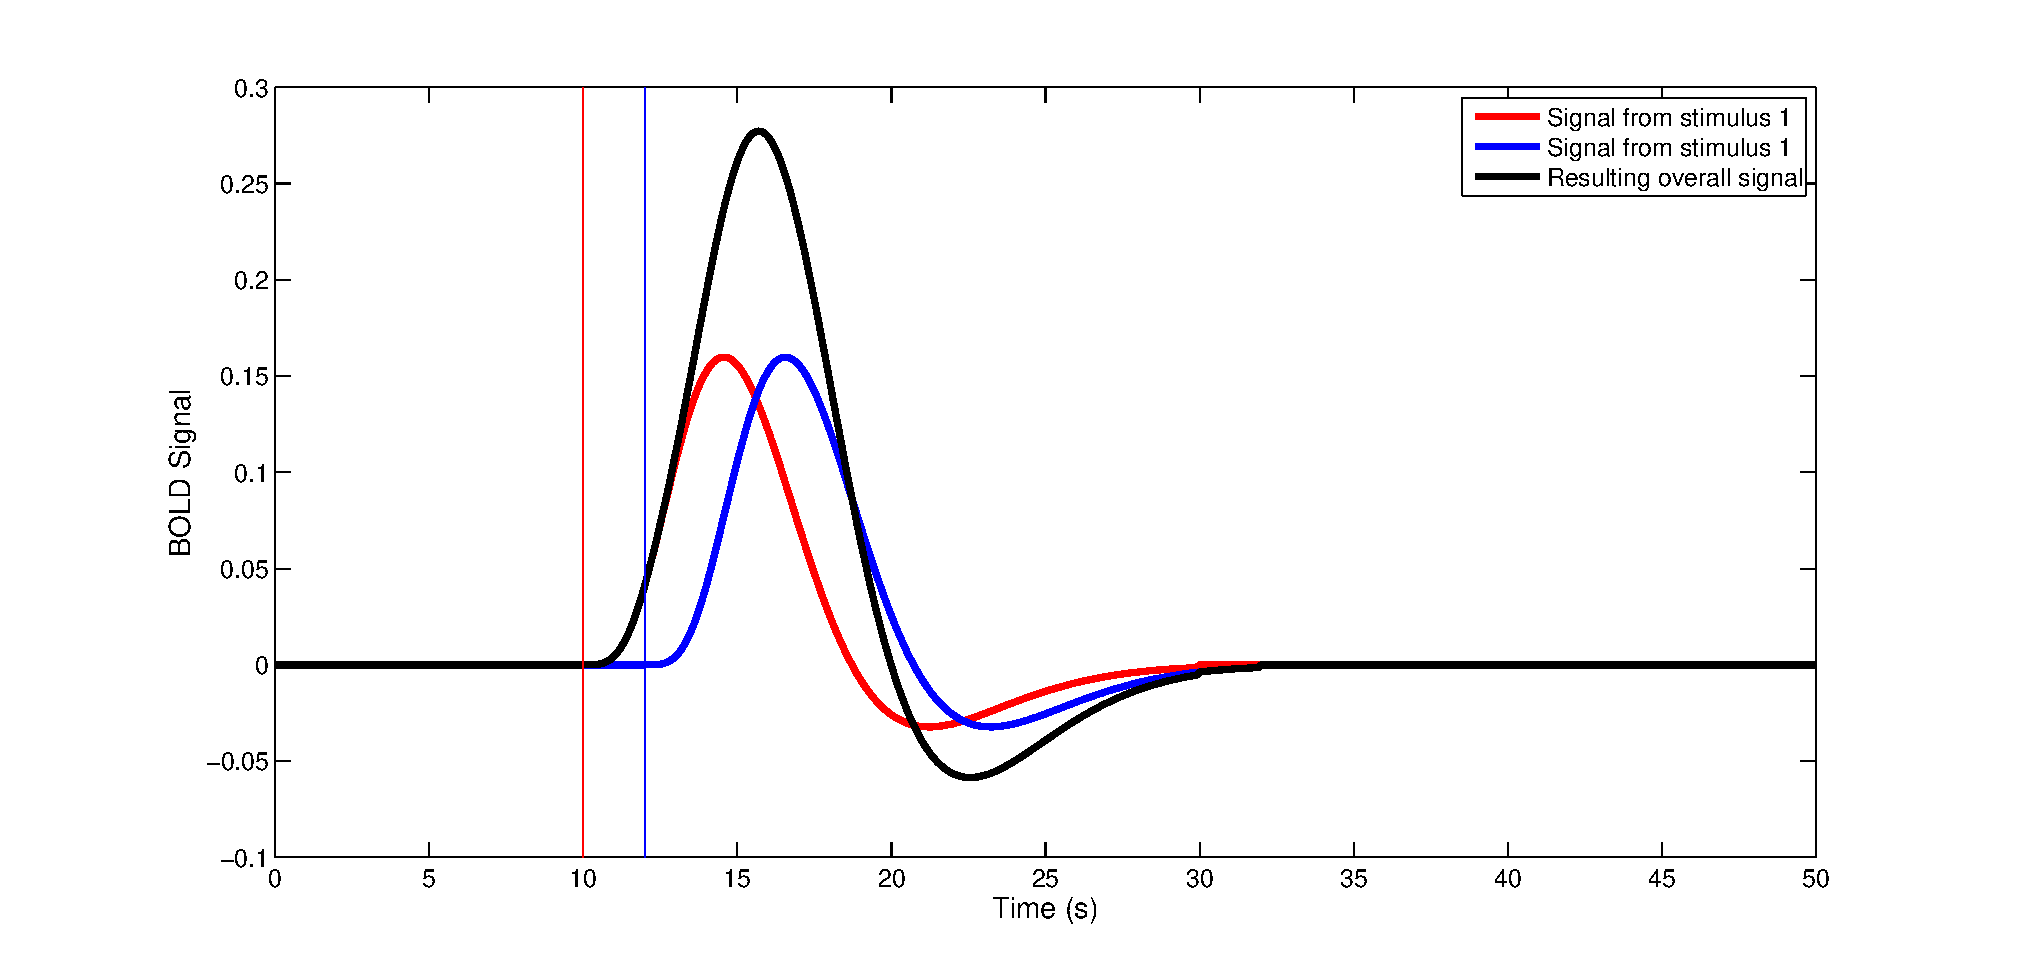
\includegraphics [scale=0.5,center] {HRF_two.eps}
    \caption{\textbf{Propiedad lineal de la HRF.} Dos estímulos (a 10 y 12 segundos) producen dos FRH (rojo y azul, respectivamente), que linealmente se unen para producir la FRH (negra) resultante que se mide.}
    \label{F:HRF_two}
\end{figure}

\begin{figure}
	\centering
    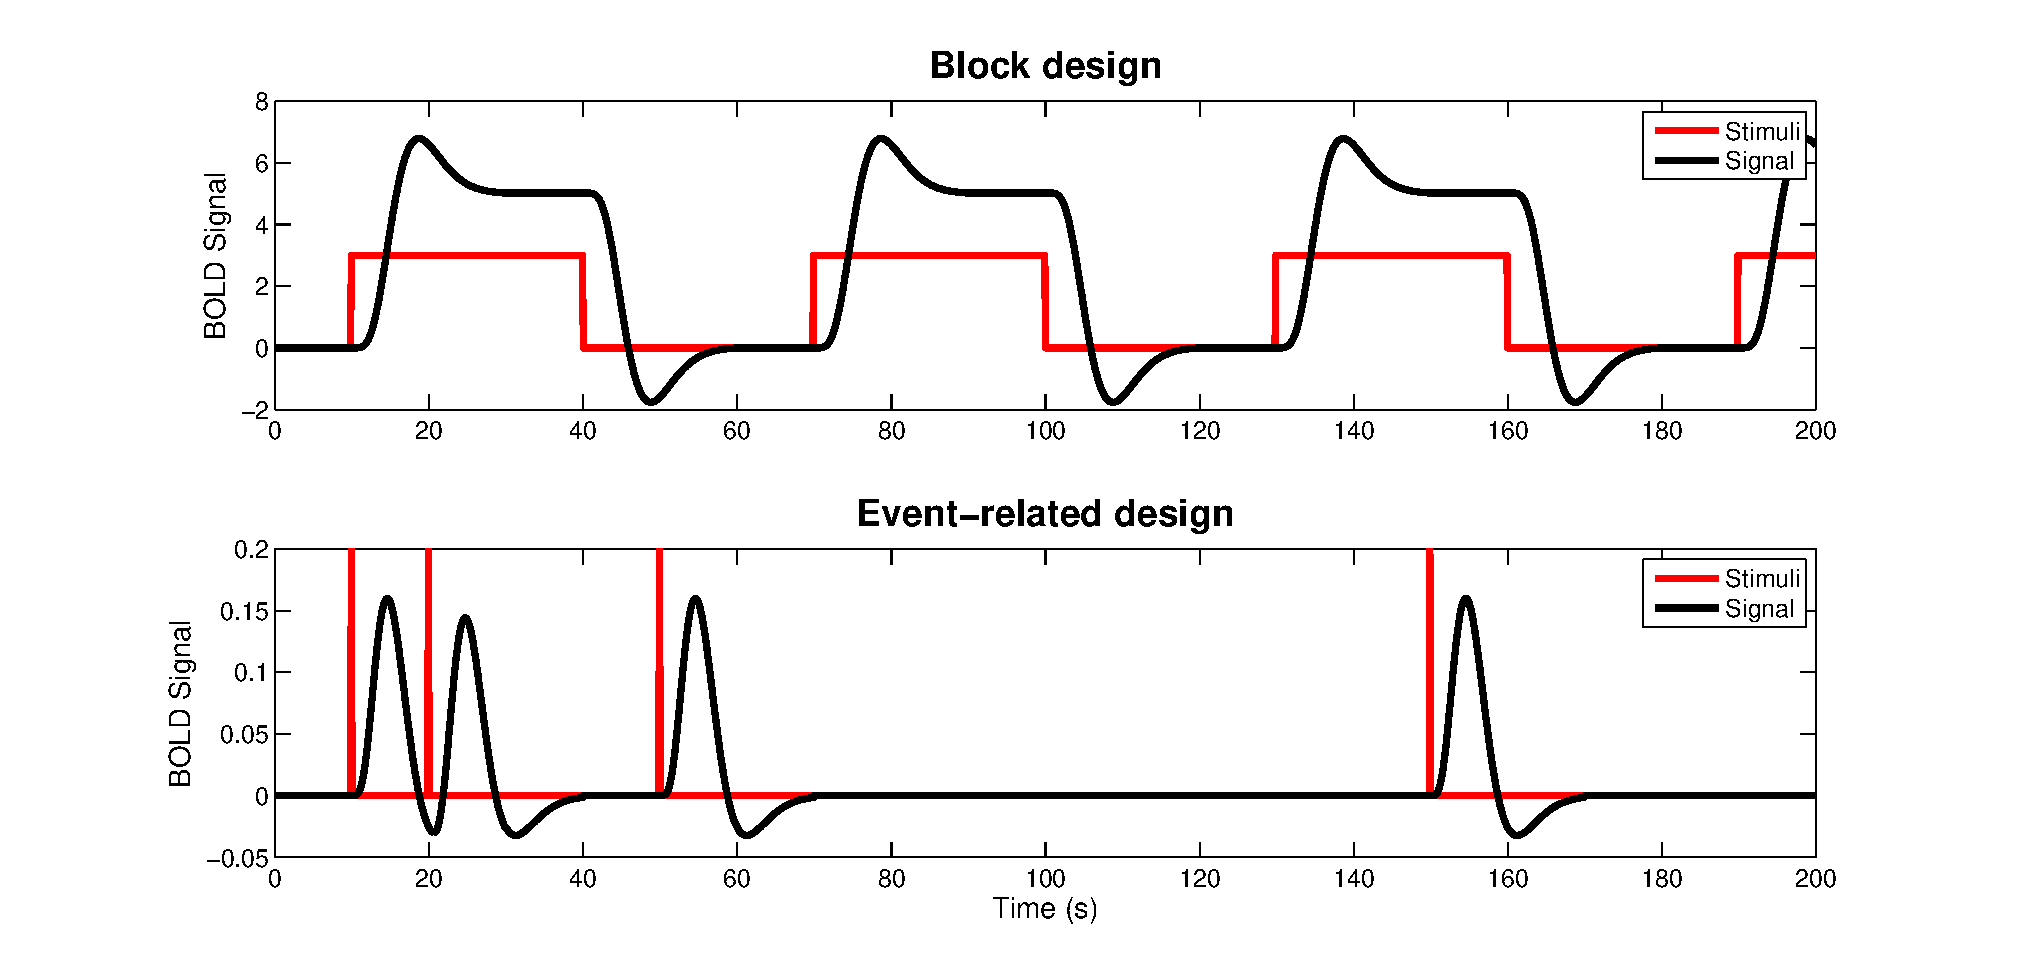
\includegraphics [scale=0.5,center] {fMRI_designs.eps}
    \caption{\textbf{Diseños de bloque (superior) y relacionados con eventos (inferior).} Las épocas de descanso de actividad están indicadas por las casillas rojas en el diseño del bloque, mientras que las líneas rojas indican el estímulo (o actividad) en el diseño relacionado con  eventos. Las líneas negras indican la señal esperada, que resulta de la convolución de la FRH (Figura 1.1) con el vector de estímulo (rojo). Observe que los diseños de bloques producen una amplitud de señal mucho mayor que los diseños relacionados a eventos, debido a la adición lineal de varios FRHs (Figura 1.2).}
    \label{F:fMRI_designs}
\end{figure}

\section{Análisis de la señal BOLD}

En el escenario más simple, podríamos restar todas las imágenes que pertenecen a los períodos de tareas de los períodos de descanso, y veríamos una señal positiva neta sólo en aquellas regiones que participan en la tarea. Sin embargo, este enfoque no tiene en cuenta la naturaleza lenta de la FRH, y no es lo suficientemente poderoso para muchos propósitos. En su lugar, podemos utilizar plenamente el modelo FRH y el hecho de que la convolución de esa función con nuestro diseño de bloque nos dará la señal esperada, entonces, todo lo que necesitamos hacer es comprobar si nuestra señal obtenida se parece a la señal predicha. Esto se logra normalmente a través del modelo lineal general (MLG), una herramienta estadística extremadamente útil. En esencia, el MLG es simplemente una forma sencilla de hacer múltiples regresiones lineales, que son el pan y la mantequilla de las estadísticas. La practicidad del MLG es que estas regresiones múltiples se realizan usando álgebra matricial. El MLG toma la forma: 

\begin{equation} 
y = \textbf{X}\beta + \epsilon 
\end{equation} 

donde \textbf{X} es una matriz que tiene tantas columnas como regresores y tantas filas como puntos de tiempo, \(\beta\) es un vector de los coeficientes por el cual tendríamos que multiplicar \textbf{X} para obtener y, y finalmente, \(\epsilon\) es el error residual, que afortunadamente es muy pequeño. En nuestro ejemplo simple de la corteza motora, \textbf{X} sólo tiene una columna, y los valores correspondientes corresponden a la convolución de la FRH con el diseño del bloque. Sin embargo, otros paradigmas más complejos pueden tener varios regresores, por ejemplo una tarea visual en la que los sujetos se muestran imágenes en bloques de diferentes categorías, por ejemplo casas, caras y símbolos; en este caso, \textbf{X} tendría tres columnas. Al ajustar el MLG a la señal, obtenemos el vector \(\beta\), y para cada uno de sus elementos podemos saber cuánto (y cuán significativamente) ese regresor particular (actividad/bloque/categoría) contribuye a la señal resultante en cada voxel. \\

\begin{figure}
	\centering
    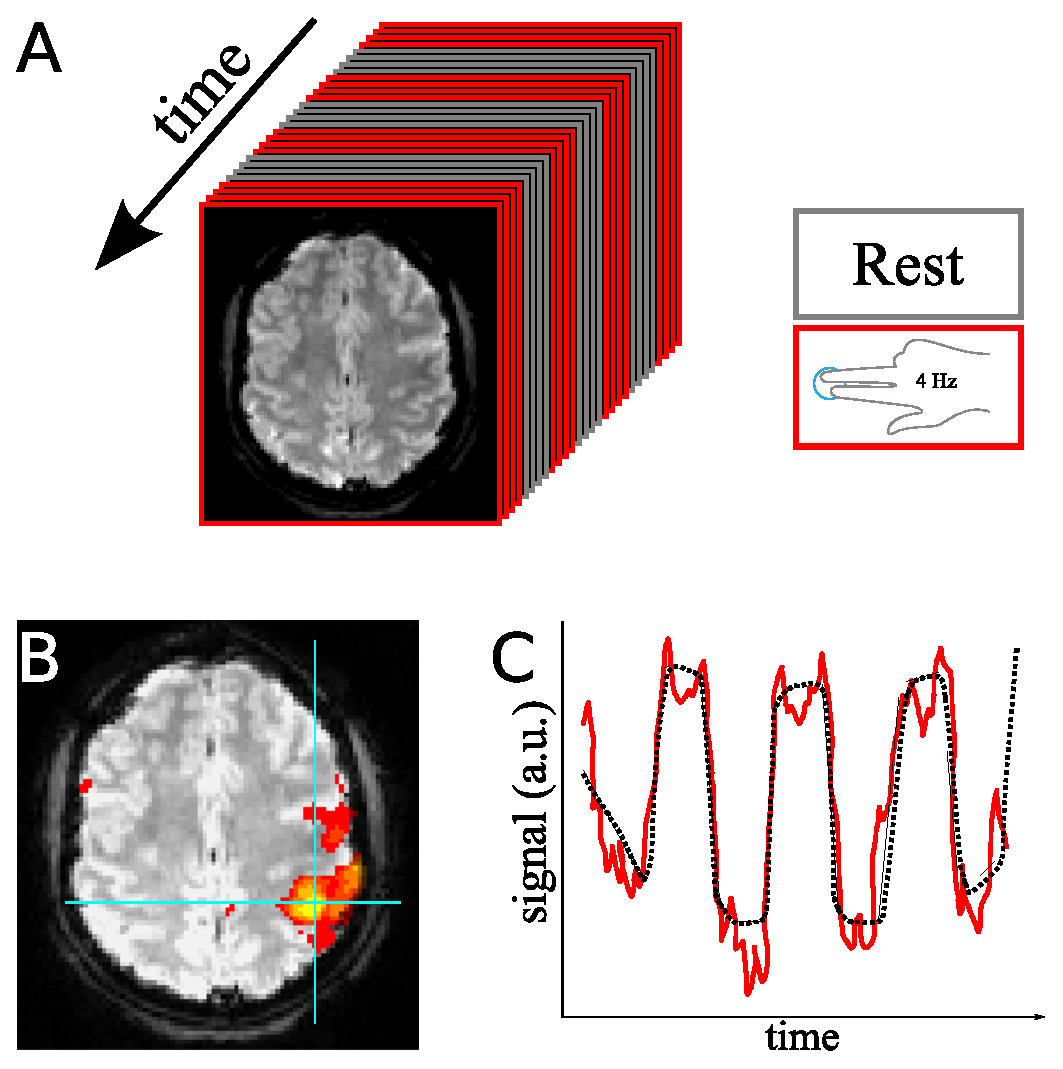
\includegraphics [scale=0.7,center] {example_fMRI.eps}
    \caption{A: Un paradigma simple para visualizar la actividad de la corteza motora. Los bloques de ``typing'' con los dedos a 4 Hz se entrelazan con bloques de descanso, cada bloque dura 30 segundos, con 5 repeticiones de cada bloque. B: En cada voxel, el modelo lineal general se ajusta a la señal, y sólo aquellos voxels que muestran un buen ajuste (por debajo de cierto umbral de valor p) están coloreados en colores cálidos. C: La señal (roja) del voxel en el centro de la mira en B se muestra a lo largo del tiempo, y coincide estrechamente con el comportamiento esperado (negro punteado), que resulta de la convolución de un FRH canónico con los bloques prescritos en el paradigma.}
    \label{F:example_fMRI}
\end{figure}

Observe, sin embargo, que al ajustar el MLG en una base voxel por voxel, debemos asegurarnos de que la misma posición espacial corresponda a la misma estructura cortical a lo largo del tiempo. Desafortunadamente (o afortunadamente, en otros escenarios), los sujetos vivos se mueven; éstos pueden tener movimientos voluntarios e involuntarios a través de la sesión de exploración de fMRI, y por lo tanto el voxel con coordenadas {\it x, y, z} podría corresponder al giro pre-central al inicio de la sesión y al giro post-central al final. Por lo tanto, antes de montar el MLG debemos realinear todos los volúmenes a uno solo, que puede ser el primero, el centro o el último de la serie. Esto se realiza usando un registro de cuerpo rígido con 6 grados de libertad; cada volumen se hace girar y se mueve aproximadamente hasta que la diferencia con el volumen móvil y el volumen de referencia es despreciable. La corrección de movimiento es sólo uno de los muchos pasos de preprocesamiento necesarios antes del ajuste de MLG, y otros procesos incluyen: corrección de inhomogeneidades geométricas de la imagen, corrección de tiempo de corte, extracción de cerebro (no necesitamos ajustar el MLG en el aire alrededor de la cabeza, podemos acelerar todos los cálculos), suavizado espacial, normalización de intensidad, filtrado temporal, filtro de paso alto y otros. El lector interesado debe consultar el excelente y muy práctico libro de Poldrack et al., que abarca muchos de estos aspectos \citep{Poldrack_2011}.

Una exploración típica del cerebro por IRMf puede tener decenas de miles de voxels, y para cada uno encajaremos en un modelo y realizaremos operaciones estadísticas e inferencias. Además de la potencia de cálculo necesaria, se debe considerar la aparición de resultados falsos positivos. Normalmente, cuando realizamos una inferencia estadística sobre, digamos, el peso de los niños tomados de dos escuelas diferentes, establecemos nuestro \(\alpha\) en 0,05. Es decir, si nuestra prueba {\it t} termina mostrando un valor de p mayor que 0,05, concluiremos que el peso de los niños no difiere entre estas dos poblaciones. Sin embargo, si realizamos el mismo experimento 100 veces, pero dibujando diferentes muestras de cada escuela en cada momento, podríamos encontrar que 5 de estos 100 experimentos ``demuestran'' que el peso de los niños depende de la escuela a la que asisten. Esto se conoce como un error de Tipo I, o un falso positivo\footnote{Una explicación humorística, pero formal de los errores de Tipo I se puede encontrar en http://xkd.om/882/}. La corrección de Bonferroni dicta que si realizáramos 100 experimentos separados, deberíamos establecer nuestro $\alpha = \alpha/n$ siendo {\it n} el número de pruebas realizadas. Para fines de fMRI, esto es ridículamente estricto, ya que n es del orden de decenas de miles. Además, la corrección de Bonferroni supone la independencia de las muestras entre las pruebas, algo que no podemos garantizar en IRMf: un voxel en el giro pre central es muy probable que se comporten como su vecino, que también está en el mismo giro. Con el fin de tratar con falsos positivos y todo tipo de problemas estadísticos en IRMf, una herramienta muy útil fue desarrollado para probar si ``clusters'' de voxels mostraron un comportamiento particular que no podía explicarse por casualidad. Esta herramienta es la teoría de campo aleatorio \citep{Worsley_1999}. Puesto en términos muy simples, si los positivos falsos son aleatorios, entonces su distribución espacial también debe ser aleatoria; la probabilidad de encontrar varios falsos positivos agrupados es baja (Figura 1.5). Esta teoría trata de encontrar lo improbable que es encontrar estos clusters, y asigna un valor p (corregido) para cada grupo de activación. Herramientas estadísticas como el MLG y la teoría del campo aleatorio son extremadamente útiles para los análisis IRMf, que es un método intrínsecamente ruidoso. Considérese, por ejemplo, que los cortices primarios muestran cambios en la señal BOLD en el rango del 1-4\% entre los períodos de tarea y descanso, mientras que los cortices de asociación y las regiones involucradas en procesos cognitivos pueden mostrar cambios de menos del 1\% entre las condiciones.

\begin{figure}
	\centering
    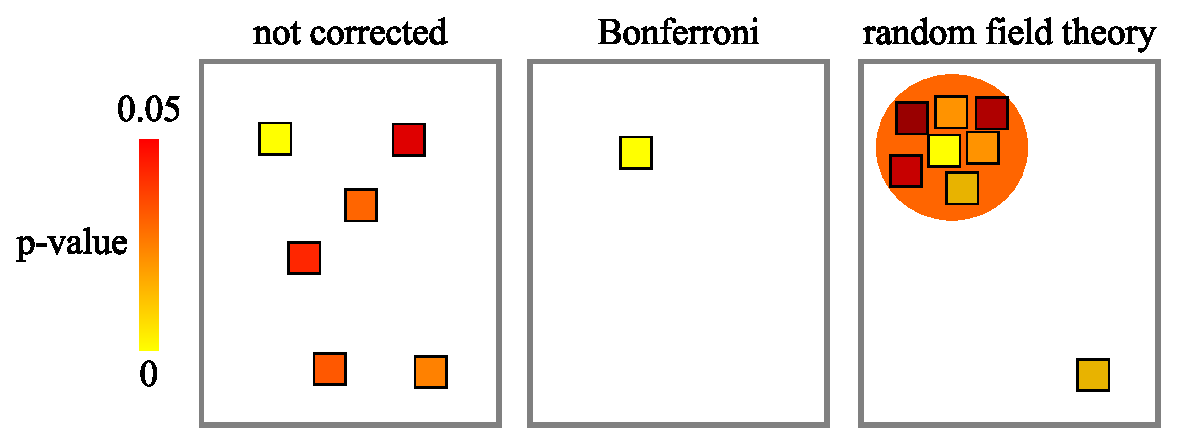
\includegraphics [scale=0.7,center] {RFT.eps}
    \caption{\textbf{Representación caricaturizada de la teoría de campos aleatorios.} Si no se corrige para comparaciones múltiples, podrían surgir varios hallazgos falsamente positivos, pero deberían tener una distribución espacial aleatoria. La corrección por el método de Bonferroni es estricta y sólo una de nuestras pruebas sigue siendo estadísticamente significativa, a expensas de la pérdida probable de otros positivos verdaderos. Es improbable que los falsos positivos ocurran en proximidad espacial cercana, y la teoría de campo aleatorio asigna un valor p (corregido) para un ``racimo'' (círculo naranja) de pruebas que superan un umbral estadístico dado (no corregido). Los falsos positivos aislados se descartan (cuadro inferior derecho).}
    \label{F:RFT}
\end{figure}

\section{Análisis de IRMf en grupo}

Hasta ahora hemos considerado un análisis de un solo sujeto de la señal BOLD. Sin embargo, es muy probable que queramos probar si una región en particular está involucrada en una determinada tarea en una gran muestra de sujetos, tratando de generalizar a toda la población. Sin embargo, la anatomía del cerebro, aunque muy similar entre los sujetos, no es idéntica. Si vamos a hacer análisis voxel por voxel, entonces debemos tratar de hacer que los cerebros entre sujetos sean lo más parecidos posible. Hay muchos acercamientos a este problema pero, en general, cada cerebro es realineado y ``deformado'' para parecer un solo cerebro o un atlas cerebral sintético. El atlas cerebral más utilizado es derivado del Consorcio Internacional para el Mapeo Cerebral (ICBM), para el cual hay varias versiones. La forma en que se lleva a cabo está fuera del alcance de este documento.

En los análisis de grupo también debemos asegurarnos de que las unidades en las que medimos cualquier cosa son las mismas entre todos los sujetos. Como vimos en la Figura 1.4, generalmente usamos unidades arbitrarias para medir la señal BOLD, que por supuesto no podría ser un buen candidato. Lo que podemos hacer, en cambio, es ajustar el MLG en cada sujeto primero, y obtener el \(\beta\) correspondiente para el regresor de interés. A continuación, este mapa de imagen \(beta\) se deforma al atlas de referencia, y estos mapas se concatenan en la 4ª dimensión, donde ``tiempo'' es sustituido por ``sujeto''. Ahora es posible ajustar el MLG de la misma manera que lo hicimos para el caso de un solo sujeto, pero lo que estamos buscando ahora es si el regresor en cuestión es relevante para la señal BOLD, en promedio, evaluado en un grupo de sujetos. Se pueden hacer otras inferencias estadísticas, como si la señal BOLD está modulada, en promedio, por un regresor en comparación con otro regresor (véase, por ejemplo, la Figura 1.6).

\begin{figure}
	\centering
    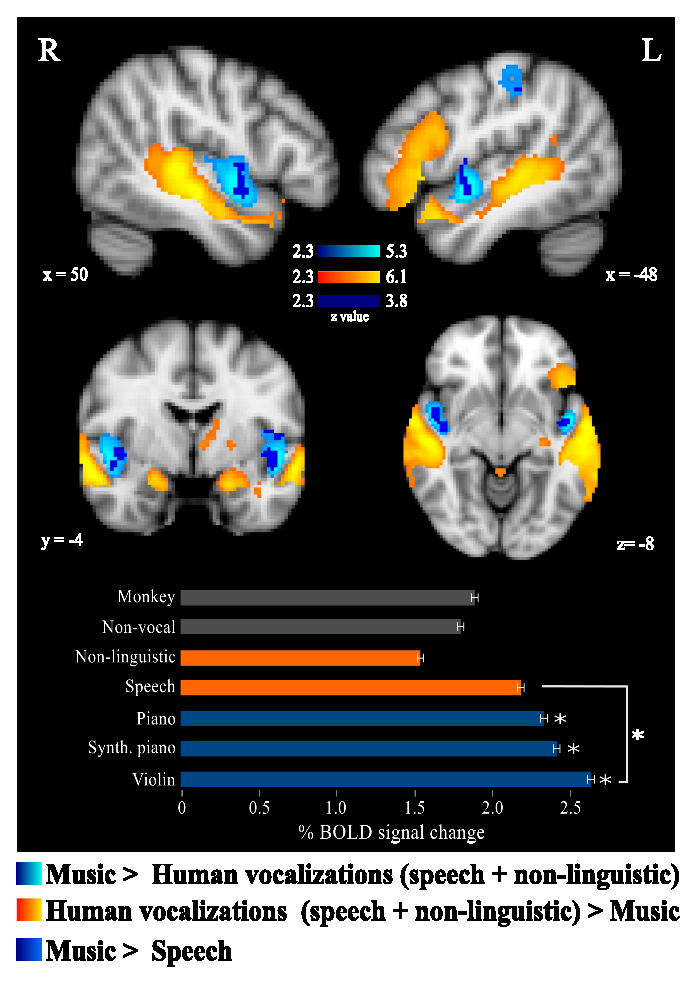
\includegraphics [scale=1,center] {Arafat_Figure3.eps}
    \caption{\textbf{Ejemplo de un resultado IRMf de un grupo de 53 sujetos.} Cada participante escuchaba bloques de estímulos acústicos que formaban parte de una de varias categorías (fragmentos de música interpretados en piano o violín, fragmentos de voz, vocalizaciones no lingüísticas, sonidos no vocales y vocalizaciones de mono). Los colores cálidos muestran regiones corticales con mayor señal BOLD durante el habla o vocalizaciones no lingüísticas, en comparación con fragmentos musicales. Los colores fríos muestran el contraste opuesto, con el azul oscuro mostrando que la música provoca un contraste mayor que el habla. Las barras de error en la parte inferior muestran el cambio medio de la señal porcentual para cada categoría en un voxel dentro del racimo azul. Tomado de Angulo-Perkins et al. \citep{Angulo_2014}}
    \label{F:Arafat_Figure3}
\end{figure}

\clearpage
\thispagestyle{plain}

\newpage
\chapter{IRM por Difusión y Tractografía}

Este capítulo se toma en gran parte de la tesis doctoral del autor. University of Alberta, 2007. Texto completo disponible en personal.inb.unam.mx/lconcha

\section{Difusión de moléculas de agua}

Todas las moléculas con una temperatura por encima del cero absoluto (es decir, $>$-273.15 \textdegree{}C) están en movimiento constante. Este fenómeno fue descrito por primera vez en 1828 por Robert Brown \citep{Brown_1828}, basado en la observación del movimiento aleatorio de los granos de polen suspendidos en el agua. Aunque los granos de polen son considerablemente más grandes que las moléculas individuales, el comportamiento descrito por Brown es similar al observado en las moléculas \footnote{De hecho, el movimiento de los granos de polen fue secundario a la difusión del agua moléculas en las que fueron suspendidas.}, por lo tanto, el fenómeno molecular se denomina comúnmente movimiento browniano. La difusión es accionada térmicamente y en el caso más simple es completamente estocástica, con cada molécula describiendo una ``caminata aleatoria'' en el tiempo. Por ejemplo, si una sola molécula de agua suspendida en un mar infinito de agua tranquila pudiera ser seguida a través del tiempo, el camino parecería ser completamente al azar, con probabilidades iguales de ir a cualquier lugar en cada paso del tiempo. Cuanto más tiempo observamos, más lejos podría estar la molécula de agua desde donde comenzó. Sin embargo, con probabilidades iguales de moverse en cualquier dirección, el desplazamiento promedio en el tiempo sería cero.

Albert Einstein resolvió matemáticamente las observaciones de Brown \citep{Einstein_1905}. Consideremos varias moléculas de agua que se difunden libremente, cada una con una posición inicial {\it r} en el tiempo {\it t = 0}. Si permitimos que se difundan durante un período de tiempo \(\tau\), cada molécula de agua estará entonces en la posición {\it r'}. El coeficiente de difusión {\it D} se puede encontrar por:

\begin{equation}
D = \frac{1}{6 \tau}  \langle \textbf{R}^T\textbf{R} \rangle
\end{equation}

donde \textbf{R} = {\it r'- r}. El desplazamiento del giro en el tiempo se considera sobre el conjunto de giro (soportes angulados). El desplazamiento cuadrático medio en el tiempo {\it t} está dado por:

\begin{equation}
rms_{n} = \sqrt{2nDt}
\end{equation}
donde {\it n} es el número de dimensiones. El desplazamiento de moléculas de agua en una dimensión se ejemplifica en la Figura 2.1. \\

\begin{figure}
	\centering
    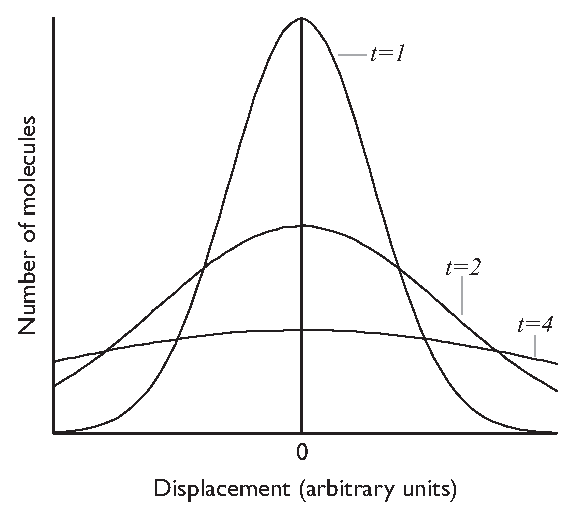
\includegraphics [scale=1,center] {gaussianDiffusion.eps}
    \caption{\textbf{Desplazamiento unidimensional de moléculas de agua en el tiempo.} Un número arbitrario de moléculas de agua con posición = 0 en {\it t} = 0 se difunde con el tiempo. El perfil de desplazamiento gaussiano se amplía a medida que pasa el tiempo.}
\end{figure}

Recuerde que la difusión es aleatoria (es decir, isotrópica) y, por lo tanto, {\it D} es independientemente recta. La magnitud de {\it D} depende de la viscosidad y temperatura del medio, y del tamaño de la molécula. {\it D} de agua a 37 \textdegree{}C es alrededor de 3,04×10\textsuperscript{-3} mm\textsuperscript{2}/s \citep{Mills?1973}.

En el caso de las moléculas de agua, el soluto y el disolvente son la misma molécula, y el fenómeno se denomina autodifusión, para lo cual el modelo de caminata aleatoria simple puede predecir adecuadamente su comportamiento. Ejemplos de auto-difusión de las moléculas de agua se pueden ver en la Figura 2.2. Para el resto de este documento, el término {\it difusión} se utiliza para referirse a la auto-difusión de moléculas de agua.

\begin{figure}
	\centering
    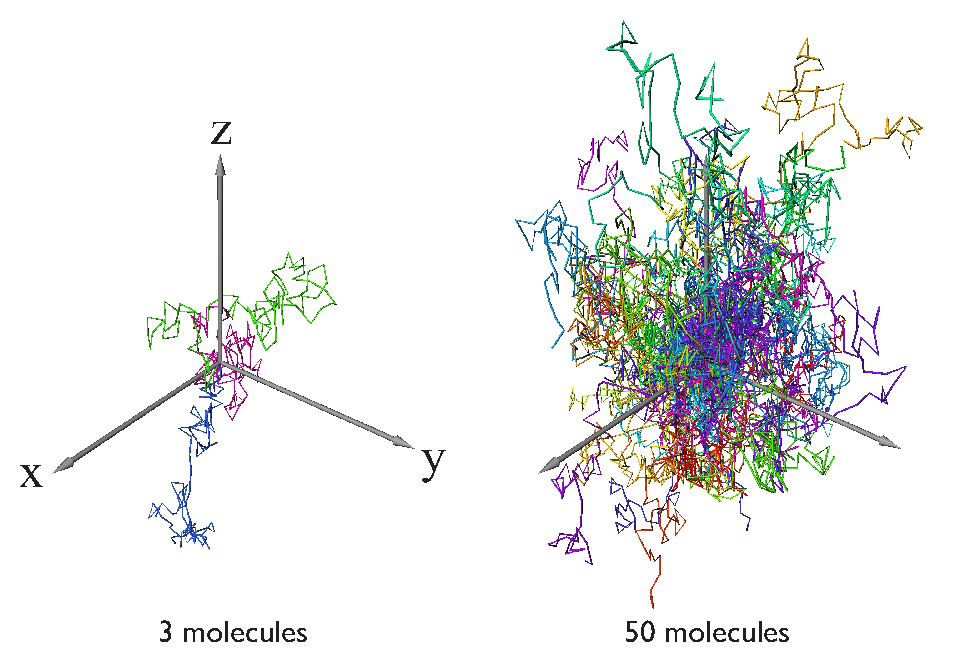
\includegraphics [scale=0.9,center] {isotropicExamples.eps}
    \caption{\textbf{Simulación de caminata aleatoria sobre 100 pasos de tiempo de 3 y 50 moléculas de agua.} La dirección de cada molécula se define aleatoriamente en cada paso del tiempo. Con el tiempo, las moléculas de agua tienen una probabilidad no nula de visitar cualquier posición en el espacio, pero, en promedio, han movido poco (si es que hay alguna) del origen.}
\end{figure}

\subsection{Medición de la difusión con resonancia\\ magnética nuclear}

Los efectos de la difusión sobre la señal de RMN se conocen desde la década de 1950, cuando el spin-eco fue descrito por Hahn \citep{Hahn_1950}. Algunos años más tarde, Carr y Purcell publicaron su trabajo sobre medidas cuantitativas T2, en las que reconocen la importancia de la difusión e incluso miden {\it D} de una muestra de agua \citep{Carr_1954}. En 1956, Torrey modificó las ecuaciones de Bloch para incluir un término de difusión \citep{Torrey_1956}. Estos primeros intentos de medir {\it D} se basaron en el uso de una perturbación constante del campo magnético principal que, entre otros problemas, dificultó la distinción de los efectos relacionados con el {\it D} de la relajación transversal.

Sin embargo, fue el trabajo de Stejskal y Tanner \citep{Stejskal_1965} en los años sesenta lo que facilitó la medición cuantitativa de los coeficientes de difusión molecular mediante el uso de una secuencia de eco de spin de gradiente pulsado (PGSE). La idea básica es codificar la posición espacial de las moléculas de agua (spins) en {\it t} = 0, invertir la fase de spin con un pulso \(\pi\) y decodificar la posición del spin después del tiempo \(\tau\). La posición de giro es codificada y recodificada con el uso de gradientes de campo magnético (Figura 2.3). Con más detalle: Después de la aplicación de un impulso de radiofrecuencia $\pi/2$ que coloca la magnetización neta en el plano {\it x, y} con fase cero, se activa un gradiente de campo magnético con amplitud {\it G} y duración \(\delta\), lo que imparte una fase a los giros según su posición espacial. Un \(\pi\) impulso de radiofrecuencia invierte entonces la fase de las vueltas. Un segundo gradiente de campo magnético con las mismas características que el primero (con una separación de ${\it tiempo} = \Delta$) hace que los giros no móviles recuperen su fase original. La señal NMR (echo) se adquiere en este punto. Si los giros se mueven durante el tiempo entre los dos gradientes del campo magnético (debido a la difusión o a cualquier otra causa), los giros no volverán a fase completamente, lo que hace que se obtenga menos señal de RMN. Obsérvese que los gradientes de campo se aplican linealmente en una dimensión, proporcionando sensibilización a la difusión sólo a giros que se mueven en esa dirección particular. Es decir, si un giro se mueve perpendicularmente a la dirección del gradiente del campo, no contribuirá a la pérdida de la señal de RMN. La señal puede ser adquirida a través de un eco de spin, como se ha descrito anteriormente, o a través de un eco estimulado \citep{Tanner_1970}. Este último enfoque, que está fuertemente ponderado a T1, minimiza la pérdida de señal a través de la relajación transversal, aunque su propia naturaleza se traduce en una reducción del 50\% de la señal original disponible.

Mediante la modificación de las características de la secuencia ``PGSE'', se puede aumentar o disminuir la sensibilidad a la difusión. Si la amplitud de los gradientes se incrementa {\it (G)}, los giros requerirán menos movimiento para experimentar un campo magnético diferente, aumentando así el cambio de fase. Alternativamente, se puede permitir que los giros se difundan durante un período de tiempo más largo, aumentando la probabilidad de que los giros se desfasen. El tiempo de difusión se expresa como $\Delta - \delta/3$, donde la corrección $\delta/3$ explica la difusión que se produce durante el tiempo en que los gradientes se activan \citep{Stejskal_1965}. La sensibilidad a la difusión se expresa como:

\begin{equation}
b = \gamma^2G^2\delta^2 (\Delta - \frac{\delta}{3})
\end{equation}

\begin{figure}
	\centering
    \includegraphics [scale=0.6,center] {stejskal_sequence.eps}
    \caption{\textbf{Secuencia de eco de giro de gradiente pulsado.} La posición espacial de las moléculas de agua se codifica como fase mediante el uso de un gradiente de campo magnético con duración \(\delta\) y magnitud {\it G}. Un pulso \(\pi\) invierte la fase de espín. Un segundo gradiente de campo magnético, idéntico al primero, reenfoca la fase de todos los giros estacionarios. Los giros móviles no experimentan el mismo campo magnético antes y después del impulso de reorientación y el conjunto no se reenfoca homogéneamente, dando como resultado la pérdida de la señal. La modificación de esta secuencia, utilizada en este documento, se presenta en la Figura 2.20.}
    \label{F:stejskal_sequence}
\end{figure}

donde \(\gamma\) es la relación giromagnética de protones de hidrógeno (42,58 MHz/T). La ecuación 2.3 supone que los gradientes de campo local (independiente de los gradientes de difusión-sensibilización) son mínimos en la muestra. En áreas de grandes diferencias de susceptibilidad magnética, se inducen gradientes de campo magnético local. Los gradientes locales impartirían más desplazamientos de fase al spin que no serían totalmente recuperados por el segundo pulso de gradiente, confundiendo la medición de {\it D}. Cualquier otro gradiente de campo magnético o inhomogeneidad presente durante la secuencia de ``PGSE'' debe estar presente e igual durante ambos gradiente de sensibilización de difusión pulsos con el fin de inferir correctamente {\it D}. El límite de tejido entre el aire y el tejido es un ejemplo de este problema. Afortunadamente, estos efectos están localizados (más sobre esto en la Sección 2.5.2). Los gradientes sensibilizadores de difusión no tienen que ser rectangulares, como se expresa en la ecuación anterior, en cuyo caso el área del pulso debe ser igual a la del impulso rectangular ideal. El uso de pulsos de gradiente no rectangulares no afecta a la medición de {\it D} \citep{Price_1991}.

La cantidad de señal de RMN disponible en un experimento sensible a la difusión decae exponencialmente de acuerdo con {\it D} (Figura 2.4), y se expresa como:

\begin{equation}
\frac{S}{S_0} = e^{-bD}
\end{equation}

donde {\it S} es la intensidad de señal obtenida con el gradiente de difusión activado y ${\it S}_0$ es la intensidad de señal correspondiente obtenida sin el uso de gradientes sensibilizadores de difusión. Esta ecuación también puede escribirse como:

\begin{equation}
ln (\frac{S}{S_0}) = -bD
\end{equation}\\

\begin{figure}
	\centering
    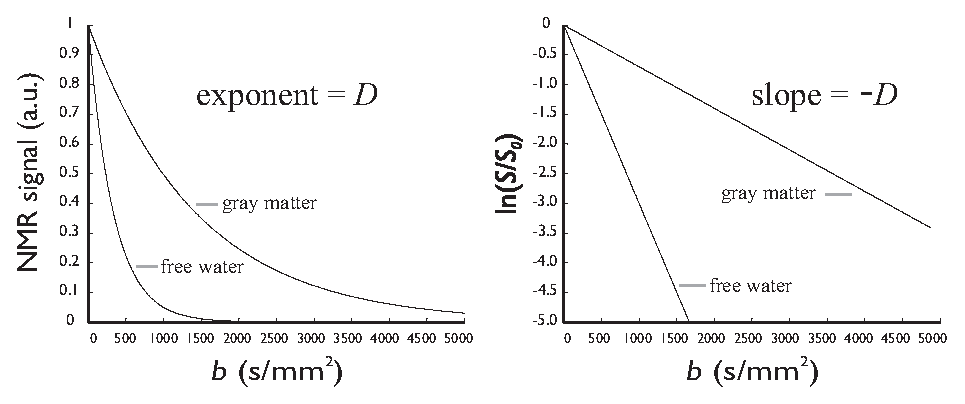
\includegraphics [scale=0.9,center] {expDecay_signal_b_2panels.eps}
    \caption{\textbf{Señal de RMN frente a sensibilización por difusión.} La señal de RMN se representa como una función de {\it b} (ecuaciones 2.4 y 2.5) para la sustancia gris ({\it D} = 0.7×10\textsuperscript{-3} mm\textsuperscript{2}/s y agua libremente difundida a 37\textdegree{}C ({\it D} = 3×10\textsuperscript{-3} mm\textsuperscript{2}/s).}
    \label{F:expDecay_signal_b_2panels}
\end{figure}

Aunque originalmente se desarrolló para medir {\it D} en muestras, el ``PGSE'' y sus variantes pueden usarse en IRM. En este caso, el volumen de interés se divide en {\it n} píxeles (elementos de imagen en el caso bidimensional) o voxels (elementos de volumen, en el caso tridimensional), y el coeficiente de difusión se puede calcular en cada píxel individual o voxel Este enfoque se conoce como difusión ponderada de imágenes (IPD) \citep{Wesbey_1984} y ahora se utiliza de forma rutinaria en la detección de lesión cerebral isquémica \citep{Sotak_2002}. Los gradientes de sensibilización a la difusión, así como los impulsos de radiofrecuencia, deben estar encendidos durante un cierto tiempo, proporcionando un tiempo de difusión efectivo $\Delta - \delta/3$) que es de alrededor de 50-100 ms. En los tejidos biológicos, la difusión de las moléculas de agua depende no sólo de la viscosidad y la temperatura, sino también de las barreras semipermeables como las membranas celulares. Para medir la viscosidad, el tiempo de difusión debe ser muy corto, limitando las interacciones entre las moléculas de agua y las barreras semipermeables. Tales cortos tiempos de difusión son difíciles de alcanzar ya que requieren gradientes muy fuertes que se aplicarán durante un corto período de tiempo \(\delta\)). Tanner y Stejskal reconocieron el efecto de las barreras de difusión y fueron los primeros en proponer la idea de medir la difusión restringida de moléculas de agua al variar el retardo entre los pulsos de gradiente \citep{Tanner_1968}. Por esta razón, el término Coeficiente de Difusión Aparente (CDA) se utiliza cuando se hace referencia a {\it D} en los tejidos biológicos, medido con RMN. Sin embargo, esto está lejos de ser un inconveniente, ya que la parte {\it aparente} de CDA es lo que nos permite hacer inferencias sobre la microestructura de los tejidos.

\subsection{Difusión de agua en el cerebro}

Con el fin de comprender el comportamiento de la difusión de agua en el cerebro, debemos discutir brevemente las propiedades básicas de los cuatro tipos principales de tejidos que residen en la cavidad intracraneal:

\begin{description}
\item[Materia gris (MG)] Este tejido contiene los cuerpos neuronales y las células gliales. Tiene un color gris-marrón, de ahí su nombre, y se distribuye en la superficie de los hemisferios cerebrales y cerebelo, así como los núcleos subcorticales (tálamo, caudado, etc.). Se compone de más de 100 000 millones de neuronas, y un número aún mayor de células gliales. Alrededor del 90\% de todas las neuronas del cerebro residen en la corteza cerebral \citep{Pakkenberg_1997}, que tiene un ancho de alrededor de 1-5 mm y se organiza en capas. Representa el 45\% del volumen total del cerebro en la edad adulta joven \citep{Rengachary_2004}.
\item[Materia blanca (MB)] Compuesta de axones y oligodendrocitos, proporciona conexiones entre porciones cercanas y distantes del cerebro. Su color es debido al contenido de mielina. En adultos jóvenes, tiene un volumen aproximado de 450 cm\textsuperscript{3} (35\% del volumen cerebral) y los axones mielinizados por sí solos representan más de 118 000 km \citep{Tang_1997}.
\item[Fluido cerebro-espinal (LCE)] Con un volumen total inferior a 150 ml, este líquido transparente baña el cerebro y la médula espinal, siendo intercambiado completamente 3-4 veces al día. Es 99\% de agua, y tiene menos de 10 células por mm\textsuperscript{3} \citep{Kandel_2000}. Representa el 10\% del volumen cerebral total \citep{Rengachary_2004}.
\item[Sangre] El flujo sanguíneo a través del cerebro entero en un adulto joven es del 15-20\% del gasto cardíaco, entre 750-1000 ml/min \citep{Kandel_2000}. Representa alrededor del 10\% del volumen total del cerebro \citep{Rengachary_2004}.
\end{description}

La difusión de agua no es completamente libre en los sistemas biológicos, debido a la presencia de membranas celulares y orgánulos, así como a la arquitectura tisular característica. Estas características significan barreras a la difusión y causan {\it anisotropía} (es decir, la difusión no es igual en todas las direcciones). La materia blanca en el cerebro, que consiste en varios haces de axones que interconectan distantes porciones discretas del cerebro, muestra un alto grado de coherencia arquitectónica. Por lo tanto, también muestra el mayor grado de anisotropía en el cerebro.

Los axones con trayectorias similares se agrupan para formar fascículos (también denominados tractos o haces de fibras, Figura 2.5). Cada axón puede estar rodeado varias veces por vainas de mielina ricas en lípidos, fabricadas por oligodendrocitos. Las vainas de mielina se interrumpen periódicamente a lo largo del axón en los nodos de Ranvier, obligando a la propagación de los potenciales de acción a ser saltatorios y por lo tanto más rápido. Los axones tienen varios diámetros que varían desde $< 1 \mu$m hasta aproximadamente 15 \(\mu\)m. Dado el coeficiente de difusión de las moléculas de agua a la temperatura corporal, una sola molécula de agua puede mostrar un desplazamiento de alrededor de 10 \(\mu\)m en 50-100 ms \citep{Le_Bihan_2002}, sin duda, suficiente para que encuentre varias membranas axonales y otras barreras. La mielina, que es una bicapa lipídica, fue asumida erróneamente como la {\it única} fuente de anisotropía de difusión. La anisotropía está efectivamente presente en los nervios no mielinizados \citep{Beaulieu_1994,Gulani_2001}, pero su presencia modula el grado de anisotropía \citep{Gulani_2001,Tyszka_2006}. La presencia de anisotropía en los nervios no mielinizados apunta a membranas celulares intactas como una de las principales fuentes de anisotropía de las moléculas de agua \citep{Beaulieu_1994,Gulani_2001}. Los micro-túbulos orientados longitudinalmente dentro de los axones, así como el transporte axonal rápido, parecen estar mínimamente involucrados en la generación de anisotropía de difusión \citep{Beaulieu_1994}. Cuando los axones están organizados de forma coherente y bien ceñidos, como en los fascículos o haces, se combinan los efectos impermeables de las vainas de mielina y las membranas axonales, lo que hace que las mediciones generales de difusión de la sustancia blanca sean anisotrópicas \citep{Pierpaoli_1996,Beaulieu2002}. Los mecanismos biofísicos de la anisotropía de difusión han sido previamente revisados \citep{Beaulieu2002}.

La materia gris, aunque está organizada en capas y columnas funcionales, no muestra el mismo grado de coherencia arquitectónica que la MB. El neuropilo (las dendritas y axones que interconectan los cuerpos neuronales {\it dentro} de la corteza), en particular, está enredado y no muestra una arquitectura coherente. Por esta razón, la difusión de agua en la corteza no muestra un alto grado de anisotropía. El FCE, que es esencialmente agua, muestra una difusión rápida que es virtualmente isotrópica. Por último, la difusión del agua en la sangre es difícil, si no imposible, de medir dado el flujo rápido que ocurre simultáneamente.

\begin{figure}
	\centering
    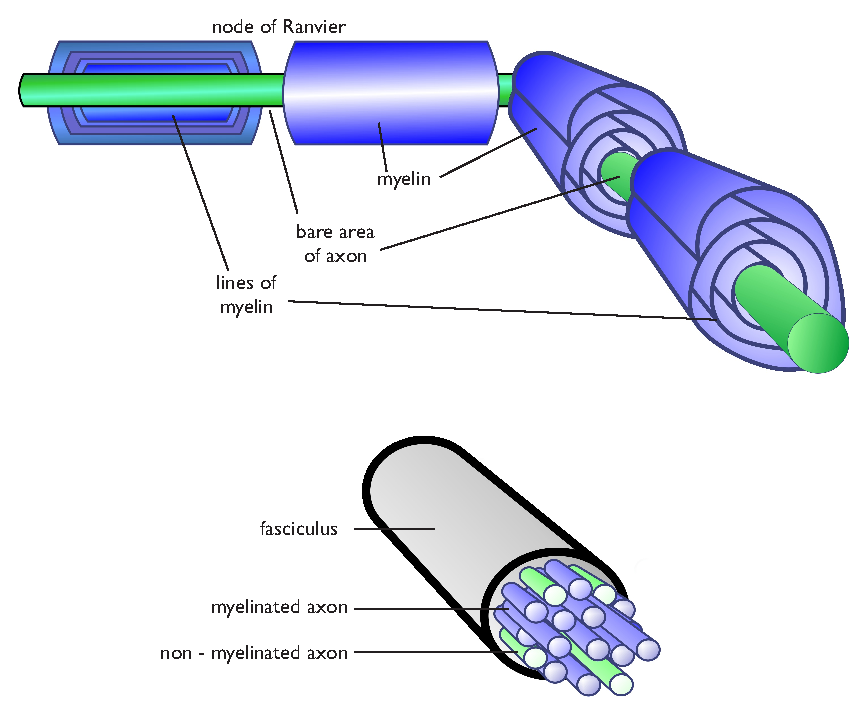
\includegraphics [scale=0.6,center] {axons2.eps}
    \caption{\textbf{Estructura básica de la materia blanca.} Algunos axones son envueltos en forma de espiral por extrusiones del citoplasma de oligodendrocitos, formando las vainas de mielina. El aislamiento de mielina se interrumpe en los nodos de Ranvier. Los axones mielinizados y no mielinizados se agrupan para formar fascículos.}
    \label{F:axons2}
\end{figure}

\section{El tensor de difusión}

Dada la anisotropía de la difusión en los tejidos organizados, una medida escalar como {\it D} no es suficiente para representar el perfil tridimensional del movimiento de las moléculas de agua. En el caso más simple, en el que se conoce {\it a priori} la orientación del tejido, tal como el nervio periférico, es posible cuantificar la anisotropía de difusión midiendo el CDA usando gradientes de sensibilización a la difusión orientados tanto en paralelo como en perpendicular al tejido y obteniendo el relación entre los dos ($\mbox{anisotrop\'ia} = (\frac{CDA\parallel}{CDA\perp})$). Sin embargo, la orientación del tejido, por lo general, no se conoce de antemano, como es el caso de la sustancia blanca. Basser y sus colegas introdujeron el formalismo del tensor de difusión en 1994 \citep{Basser_1994_2,Basser_1994}, que supera dicho problema y permite la cuantificación del CDA en cualquier dirección. Lo más importante es que el tensor de difusión proporciona información importante sobre la microestructura y la orientación del tejido organizado.

La representación tridimensional de la ecuación 2.5 es:

\begin{equation}
ln(\frac{S}{S_0}) = \sum_{i=1}^{3}\sum_{j=1}^{3} b_{ij}D_{ij}
\end{equation}

\begin{equation}
= (-b_{xx}D_{xx}+2b_{xy}D_{xy}+2b_{xz}D_{xz}+b_{yy}D_{yy}+2b_{yz}D_{yz}+b_{zz}D_{zz})
\end{equation}

en forma de matriz:

\begin{equation}
ln \bigg(\frac{S(\textbf{b})}{S_0}\bigg) = -traza(\textbf{bD})
\end{equation}

donde cada elemento en b y {\it D} corresponde a una dirección unidimensional particular de sensibilización por difusión. A partir de estas ecuaciones, el tensor puede construirse como matriz de la forma:

\begin{equation}
D
=
\begin{bmatrix}
    D_{xx} & D_{xy} & D_{xz} \\
    D_{xy} & D_{yy} & D_{zy} \\
    D_{xz} & D_{yz} & D_{zz}
\end{bmatrix}
\end{equation}

Obsérvese que {\it D} es una matriz simétrica, donde $D_{xy}, D_{xz}$ y $D_{yz}$ son repetidos en las esquinas superior derecha e inferior izquierda, ya que $D_{xy} = D_{yx}, D_{xz} = D_{zx}$ y $D_{yz} = D_{zy}$ . Si el medio es isotrópico, entonces $D{xx} = D{yy} = D_{zz}$, y los elementos fuera de la diagonal, $D_{xy}, D_{xz}$ y $D_{yz}$ son cero. Aunque puede utilizarse cualquier número ($>$ 6) de direcciones de gradiente de difusión, la mayoría de los estudios utilizan el esquema de gradiente descrito por Pierpaoli {\it et al}. \citep{Pierpaoli_1996} (mostrado en la Figura 2.6), donde {\it x}, {\it y} y {\it z} representan las bobinas de gradiente del escáner. Estos gradientes de difusión son independientes de cualquier otro gradiente necesario para la creación de la imagen (por ejemplo, gradientes de codificación de fase y frecuencia). Dicho esquema de gradiente (es decir, teniendo múltiples gradientes simultáneamente) proporciona amplitudes de gradiente resultantes que exceden la obtenida a lo largo de los ejes físicos y por lo tanto se considera ``eficiente'', ya que proporciona altos valores {\it b} en un periodo de tiempo más corto (es decir, puede ser más corto), reduciendo el tiempo de eco y la relajación de T2 durante el período de lectura (lo que produce una mayor relación señal/ruido por unidad de tiempo) \citep{Jones_2004}. Ha habido un debate considerable con respecto al número óptimo de direcciones de gradiente de difusión, con diferentes conclusiones derivadas en el marcador sustituto elegido para comparar esquemas de dirección. En términos de tener una alta probabilidad de describir con precisión la orientación del tensor, parece ventajoso utilizar más de seis direcciones, sobrestimando el cálculo del tensor \citep{Jones_2004}; por el contrario, seis direcciones parecen ser suficientes para estimar con precisión la anisotropía de difusión \citep{Hasan_2001}, siempre y cuando las direcciones del gradiente de difusión apunten a los vértices de un icosaedro, como en la Figura 2.6.

\begin{figure}
  \begin{minipage}[c]{0.45\linewidth}
    \centering%
    \begin{adjustbox}{width=\columnwidth-100pt}
    \begin{tabular}{ lll }%
      \multicolumn{3}{c}{{\it x} \hfill	{\it y} \hfill {\it z}} \\%
      \hline 
      1 & 0 &  1 \\ 
     -1 & 0 &  1 \\ 
      0 & 1 &  1 \\ 
      0 & 1 & -1 \\ 
      1 & 1 &  0 \\
     -1 & 1 &  0
    \end{tabular}%
    \end{adjustbox}
    \vspace{0pt}
  \end{minipage} 
  \begin{minipage}[c]{0.55\linewidth}
   \centering
    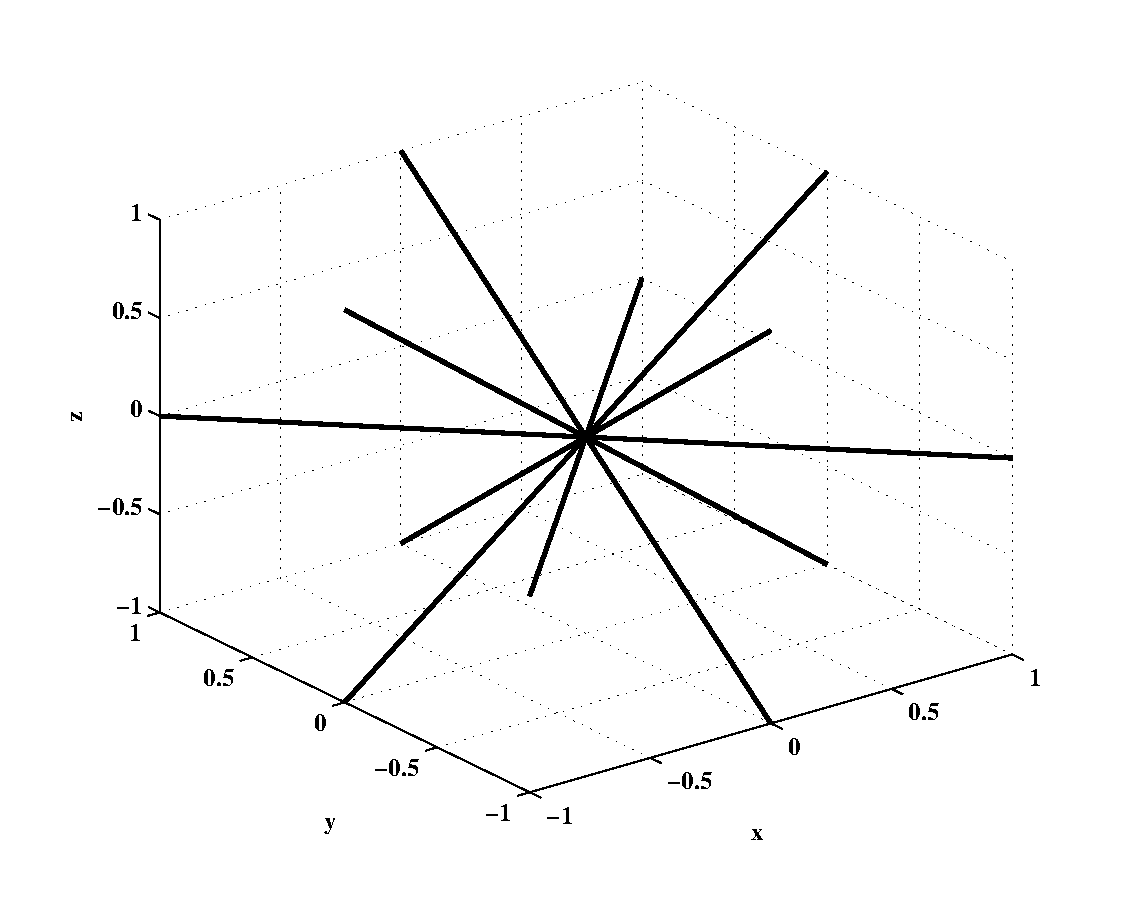
\includegraphics[width=1\textwidth, inner] {bmatrix.eps}
    \vspace{0pt}
  \end{minipage}% 
  \caption{\textbf{Direcciones de gradiente de difusión.} Las direcciones de gradiente de difusión se trazan en tres dimensiones. Las imágenes ponderadas por difusión se obtienen en seis direcciones de gradiente de difusión no planar y no colineal con el fin de obtener suficiente información para construir el tensor de difusión.}
\label{bmatrix}
\end{figure}

Una propiedad de los tensores de segundo rango es que pueden ser diagonalizados, dejando tres elementos distintos de cero a lo largo de la diagonal principal de la matriz, que se llaman valores propios. Los valores propios se ordenan según su magnitud, siendo $\lambda_{1}$ el más grande y $\lambda_{3}$ el más pequeño en magnitud. La relación matemática entre las coordenadas principales del tensor de difusión y el marco del laboratorio se describe por los vectores propios ($\nu_{1-3}$). Los ``{\it eigenvalues}'' reflejan la difusividad en una dirección dada, de acuerdo con su vector propio asociado y tienen interpretaciones biológicas directas. Por ejemplo, en el caso de la sustancia blanca, el autovalor más largo (es decir, $\lambda_{1}$) refleja el estado axonal, mientras que los valores propios asociados a ($\nu_{2,3}$) proporcionan información sobre la integridad de las vainas de mielina \citep{Song_2003,Concha_2006}).

Es más fácil entender el tensor de difusión al considerar su representación geométrica, que es un elipsoide cuyos ejes están determinados por los tres valores propios y su orientación por los vectores propios (Figura 2.7). El elipsoide puede ser conceptualizado como la superficie sobre la cual un spin en el origen se difundirá con igual probabilidad si la difusión es gaussiana. La superficie del elipsoide representa el desplazamiento difusivo cuadrático medio cuadrático del agua. La traza del tensor (traza ($\textbf {D}) = \lambda_1 + \lambda_2 + \lambda_3)$ es equivalente al tamaño del elipsoide, mientras que la difusividad media en todas las direcciones (CDA tridimensional) viene dada por:

\begin{equation}
CDA = \frac{traza (\textbf{D})}{3} = \frac{\lambda_{1} + \lambda_{2} + \lambda_{3}}{3}
\end{equation}

Los términos difusividad media (DM), {\it traza}/3 y CDA se utilizan indistintamente en la literatura. {\it Traza} CDA también se utiliza a veces para referirse a DM, aunque se refiere formalmente a DM×3.

\begin{figure}
	\centering
    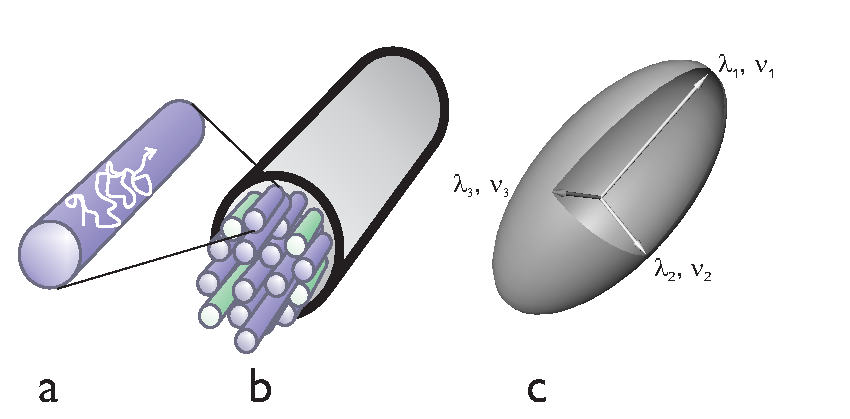
\includegraphics [scale=1,center] {DTI_ellipsoid.eps}
    \caption{\textbf{El tensor de difusión.} La difusión anisotrópica de moléculas de agua (a) en tejidos altamente organizados, como la materia blanca (b), da como resultado un tensor de difusión alargado, visualizado como un elipsoide (c). El eje mayor del elipsoide corresponde al valor propio más grande ($\lambda_1$). Por lo tanto, la difusividad principal de las moléculas de agua es paralela al vector propio correspondiente a $\lambda_1$.}
    \label{F:DTI_ellipsoid}
\end{figure}

En IPD, se utiliza un par de gradientes sensibilizadores de difusión antes del esquema de adquisición de imágenes. Las imágenes ecoplanares (IEP) \citep{Mansfield_1977,Ordidge_1988} son típicamente la secuencia de imágenes utilizada, ya que es uno de los esquemas de imagen más rápidos disponibles en la RM (se describen esquemas de imágenes alternativas en la página 46). En IEP, se utiliza un único impulso de excitación y toda la imagen se forma en menos de un cuarto de segundo. La naturaleza de un solo disparo del IEP se traduce en un solo conjunto de gradientes que se requieren para la sensibilización de difusión (Figura 2.20). Los gradientes de difusión se aplican en una dimensión (Figura 2.6), por lo tanto sensibilizando la imagen a la difusión en una dirección (además de su ponderación T2 inherente dada por los largos tiempos de eco típicamente requeridos). Las áreas de las imágenes que contienen la mayor parte de sus moléculas de agua que se difunden en una dirección que es paralela a la dirección del gradiente de difusión mostrarán una disminución de la señal, cuando se compara con la imagen ponderada no difundida. Por lo tanto, el CDA de esas regiones será alto. Por el contrario, las regiones donde la difusión es perpendicular a los gradientes de difusión no mostrará una caída tan marcada en la intensidad de la señal. Habiendo calculado el CDA sobre una base por píxel, se pueden producir mapas cuantitativos de difusividad donde la escala de grises está relacionada con CDA, como en la Figura 2.8. Es importante señalar que las áreas de hiper-intensidad visto en IPD suelen aparecer como regiones oscuras en los mapas cuantitativos CDA. Las primeras imágenes de IPD fueron presentadas en 1988 por Avram y Crooks \citep{Avram_1988}. Sin duda, la imagen ponderada por difusión ha tenido un tremendo impacto en el diagnóstico de lesiones cerebrales isquémicas, donde se ha convertido en una herramienta virtualmente indispensable \citep{Sotak_2002,Moseley_1990,Warach_1995}.\\

\begin{figure}
	\centering
    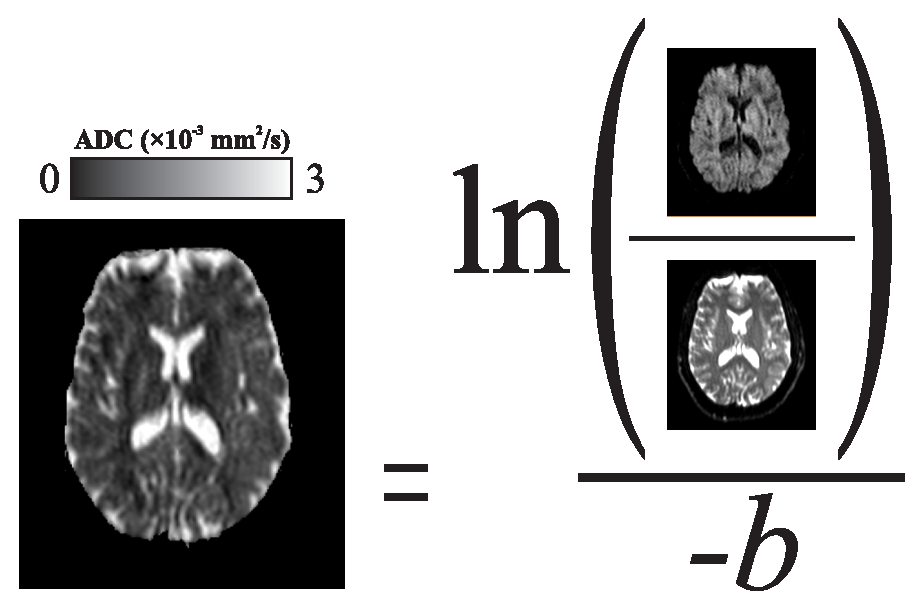
\includegraphics [scale=0.9,center] {DTI_ADCmaps.eps}
    \caption{\textbf{Mapa del coeficiente de difusión aparente cuantitativo. } El ADC se calcula sobre una base de píxel a píxel de la DWI y las imágenes ponderadas de no difusión de acuerdo con la ecuación 2.5. El gradiente de difusión se aplica en una sola dirección; $b = 1000 s/mm^{2}$. Observe la rápida difusión de FCE en los ventrículos, representada como píxeles brillantes en el mapa de ADC cuantitativo.}
    \label{F:DTI_ADCmaps}
\end{figure}

IPD es inherentemente una técnica unidimensional. Obteniendo al menos seis IPD, cada uno con una dirección de gradiente de difusión diferente (no colineal y no coplanar) (y una imagen sin sensibilización por difusión, $b = 0 s/mm^{2}$), y obteniendo sus respectivos mapas CDA en una dirección de gradiente de pixel por pixel, adquirimos toda la información necesaria para construir el tensor de difusión. El tensor se calcula de una manera pixel por pixel (Figura 2.9), dando lugar a imágenes de tensor de difusión (ITD).

\begin{figure}
	\centering
    \includegraphics [scale=1,center] {DTI_DWItoTensor.eps}
    \caption{\textbf{ Cálculo del tensor de difusión.} El tensor de difusión se calcula píxel a píxel, basado en la imagen ponderada no difundida (es decir, $b = 0 s/mm^{2}$, panel a) y seis IPD, cada uno con una dirección de gradiente de difusión diferente ($b = 1000 s/mm^{2}$, panel b). Las direcciones del gradiente de difusión se expresan como [{\it x y z}]. Observe cómo las regiones cerebrales particulares cambian el contraste dependiendo de la dirección del gradiente de difusión aplicado. Los mapas CDA individuales (no mostrados) se calculan de acuerdo con la ecuación 2.5 (véase la figura 2.8). Tras la diagonalización, los tensores de difusión resultantes se visualizan un elipsoide por píxel (ver Figura 2.7), con su intensidad de color relacionada con el grado de anisotropía (c, con región ampliada en d). Obsérvese que la orientación de los elipsoides se asemeja a la orientación esperada de la materia blanca, por ejemplo el esplenio del cuerpo calloso en d, que interconecta los dos hemisferios cerebrales. Los tensores de difusión en las cápsulas internas parecen más pequeños porque están orientados a través del plano de imagen, de acuerdo con la orientación rostro-caudal de este haz de materia blanca que demuestra la naturaleza tridimensional del tensor de difusión.}
    \label{F:DTI_DWItoTensor}
\end{figure}

Los momentos más altos del tensor de difusión proporcionan información sobre el grado de anisotropía de difusión, porque caracterizan diferentes maneras en que el tensor de difusión se desvía del caso isotrópico. Estas medidas escalares facilitan la interpretación del tensor y, derivadas de los valores propios, tienen la ventaja de ser {\it invariantes en rotación}. El caso más simple es la relación de las difusividades principales ($\lambda_{1}/\lambda_{3}$), o más intuitivamente, la relación de la difusividad paralela a la orientación del tejido ($\lambda\parallel$ frente a la difusividad perpendicular ($\lambda\perp = \lambda_{2} + 2\lambda_{3}$).

El principal inconveniente de este enfoque es que requiere la clasificación de los valores propios y, como tal, es muy sensible a las contribuciones de ruido \citep{Pierpaoli_1996}.
Otras medidas escalares de la anisotropía pueden construirse independientemente del orden de magnitud de los valores propios. La {\it relación de volumen} \citep{Pierpaoli_1996} se define como:

\begin{equation}
\textit{relaci\'on de volumen} = \frac{\lambda_{1}\lambda_{2}\lambda_{3}}{(\lambda_{1}\lambda_{2}\lambda_{3})^{3}}
\end{equation}

y representa el volumen de un elipsoide dividido por el volumen de una esfera cuyo radio es la difusividad media. Por lo tanto, los valores de Razón de Volumen van de 0 a 1, siendo 0 la anisotropía más alta y 1 el caso isotrópico completo. Debido a esto, algunos autores prefieren utilizar el término 1 - Ratio Volumen \citep{Pierpaoli_1996}.
La relación Anisotropía Relativa (RA) es otra medida de la anisotropía, que representa el coeficiente de variación de los valores propios. Esta medida se utilizó antes en la cristalografía \citep{Sands_1995}, oscila entre 0 (isotrópico) y 2 (anisotropía infinita) y se expresa como:

\begin{equation}
RA = \sqrt{\frac{1}{3}} \frac{\sqrt{(\lambda_{1} - traza (\textbf{D}))^{2} + (\lambda_{2} - traza (\textbf{D}))^{2} + (\lambda_{3} - traza (\textbf{D}))^{2}}}{traza (\textbf{D})}
\end{equation} 

Sin embargo, quizás la medida de anisotropía más utilizada es el índice de anisotropía fraccional (AF) \citep{Basser_1996}, que mide la fracción de la magnitud del tensor que se puede atribuir a la difusión anisotrópica. Va de 0 (isotrópico) a 1 (anisotropía infinita), por lo que AF más intuitiva que RA. Se define como:

\begin{equation}
FA = \frac{\sqrt{3}}{\sqrt{2}} \frac{\sqrt{(\lambda_{1} - ADC)^{2} + (\lambda_{2} - ADC)^{2} + (\lambda_{3} - ADC)^{2}}}{\lambda_1^2 + \lambda_2^2 + \lambda_3^2}
\end{equation}

Visualmente, AF se representa como elipsoides con diferentes grados de esfericidad (dado por los valores propios) como se puede ver en la Figura 2.10.\\

\begin{figure}
	\centering
    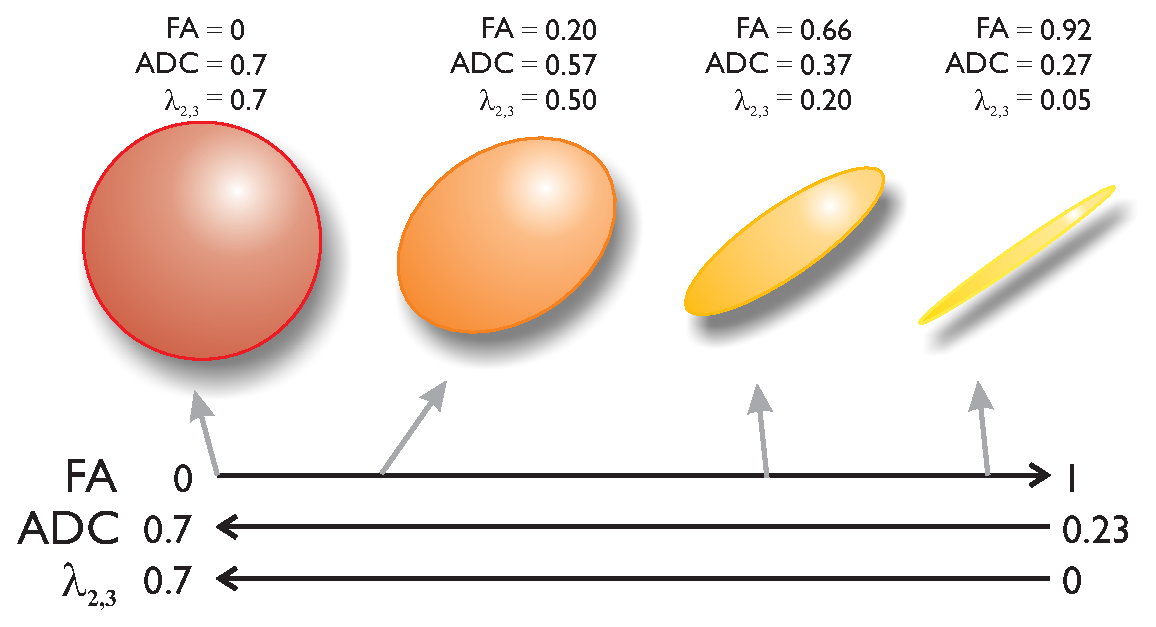
\includegraphics [scale=0.7,center] {DTI_ellipsoids_FA.eps}
    \caption{\textbf{Elipsoides tensor de difusión de diferentes grados de anisotropía.} Se muestran cuatro elipsoides del tensor de difusión que van desde isotropía pura hasta anisotropía muy alta. En todos los casos $\lambda_{1}$ se ha mantenido constante a 0,7 $× 10 - 3 mm^{2}/s$. $\lambda\perp$ (es decir, $\lambda_{2} \lambda_{3}$) se reduce progresivamente, aumentando la anisotropía y reduciendo el ADC. FA es adimensional, ADC y valores propios tienen unidades $× 10 - 3 mm^{2}/s$.}
    \label{F:DTI_ellipsoids_FA}
\end{figure}

Los índices de anisotropía cuantitativa, así como los valores propios y los componentes tensores individuales, también se pueden mostrar como mapas relacionando la intensidad de la escala de grises con la medida deseada en cada píxel (Figuras 2.11 y 2.12). De hecho, cualquier correlación de colores se puede utilizar y no se limita a una escala de grises (véase, por ejemplo, la Figura 2.9)). 

Por último, la orientación tridimensional del tensor de difusión también puede visualizarse en imágenes bidimensionales (rebanadas) utilizando diferentes aproximaciones. En el primer enfoque, ejemplificado en la Figura 2.9, se visualiza cada elipsoide de difusión (la visualización puede simplificarse mostrando cajas o líneas para representar el tensor). Este enfoque, aunque sea elegante y atractivo a la vista, es extremadamente complicado y difícil de interpretar. Otra reducción de este tema es mostrar $\nu_1$ por píxel como una ``quiver-plot''. La principal desventaja de estos métodos es que resulta difícil visualizar la orientación correcta de las flechas/elipsoides cuando están orientadas ortogonalmente al plano que se está viendo (por ejemplo, los elipsóides de difusión de la cápsula interna parecen ser isotrópicos y pequeños en la Figura 2.9 , panel d). Otros enfoques han producido mapas de escala de grises de los ángulos polares y azimutales de $\nu_1$, que requiere dos mapas para ser vistos simultáneamente \citep{Conturo_1996,Ulug_1994}. Un enfoque inteligente e intuitivo es utilizar el color para representar la orientación de los tractos de materia blanca \citep{Douek_1991,Jones_1997,Coremans_1994,Nakada_1995,Pierpaoli_1997,Jones_1997}. El método más utilizado hoy en día es el propuesto por Pajevic y Pierpaoli \citep{Pajevic_2000}. En este último método, las componentes {\it x, y} y {\it z} de $\nu_1$ se asignan a los componentes rojo, verde y azul de una imagen a todo color, respectivamente (Figura 2.13). Sin embargo, haciendo esto sólo resaltará todos los tensores en la imagen, independientemente de su anisotropía. Dado que las regiones de baja anisotropía pueden tener valores propios ligeramente diferentes sólo debido a las contribuciones de ruido, el valor propio más grande será orientado al azar \citep{Bastin_1998}. Por lo tanto, la corteza y los espacios llenos de FCE aparecerá incorrectamente tener una dirección preferida. Con el fin de superar este problema, los componentes del vector se multiplican por algún índice de anisotropía (por ejemplo, FA). Esto coincidirá con la intensidad del píxel con el grado de anisotropía, y el color reflejará la orientación del tensor; además, las regiones de baja anisotropía no abruman la imagen. Otra ventaja de este método es que la codificación de color es independientemente de la orientación de la rebanada.

El análisis del tensor de difusión no se limita a las medidas de anisotropía esbozadas anteriormente. Un método intuitivo propuesto por Westin \citep{Westin_1997} representa el tensor como una combinación de sus componentes lineal (CL), planar (CP) y esférico (CE):

\begin{figure}
	\centering
    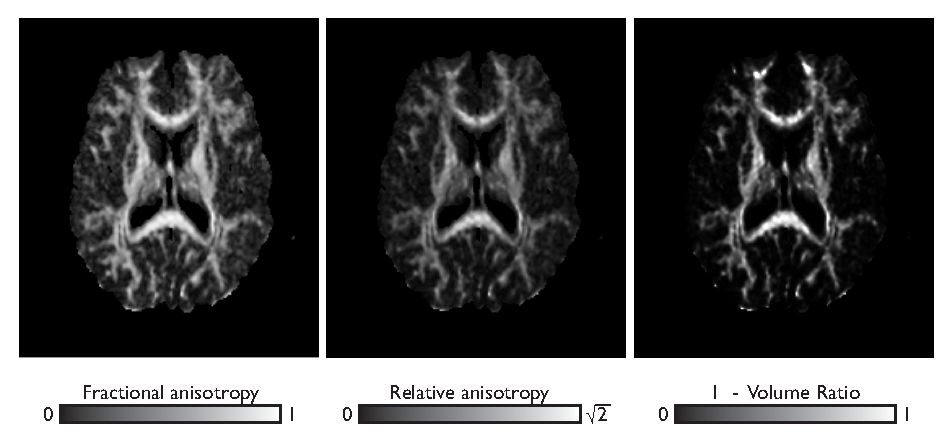
\includegraphics [scale=1,center] {DTI_quantMaps_anisotropy.eps}
    \caption{\textbf{Mapas de anisotropía de difusión cuantitativa.} Se muestran tres medidas de anisotropía de difusión. Observe cómo la sustancia blanca muestra grandes valores en los tres mapas cuantitativos, debido a su alta coherencia arquitectónica.}
    \label{F:DTI_quantMaps_anisotropy}
\end{figure}

\begin{equation}
CL = \frac{\lambda_{1} - \lambda_{2}}{\sqrt{\lambda_1^2 + \lambda_2^2 + \lambda_3^2}}
\end{equation}

\begin{equation}
CP = \frac{2(\lambda_{2} - \lambda_{3})}{\sqrt{\lambda_1^2 + \lambda_2^2 + \lambda_3^2}}
\end{equation}

\begin{equation}
CE = \frac{\lambda_{3}}{\sqrt{\lambda_1^2 + \lambda_2^2 + \lambda_3^2}}
\end{equation}

La normalización por la norma del tensor hace que cada medida oscile entre 0 y 1, y la suma de las tres medidas de forma es unidad. Cada uno de estos componentes se puede visualizar fácilmente simultáneamente usando un diagrama baricéntrico \citep{Alexander_2000}, y el índice de anisotropía total (CA) se define como la suma de las medidas de forma lineal y plana:

\begin{equation}
CA = CL + CP + 1 - CE
\end{equation}

Este método también puede ser visualizado como mapas cuantitativos (Figura 2.14). La principal desventaja del enfoque de componente de forma es su sensibilidad al ordenamiento de los valores propios, lo cual no es un problema en medidas de anisotropía como FA o RA.

\begin{figure}
	\centering
    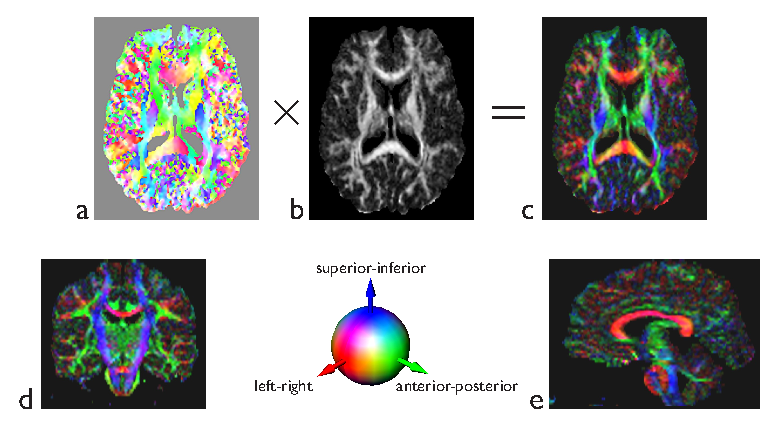
\includegraphics [scale=1,center] {DTI_colormaps.eps}
    \caption{\textbf{Mapas en color de difusividad principal.} Los componentes {\it x, y} y {\it z} del vector propio principal v 1 se asignan a los componentes rojo, verde y azul de una imagen a todo color (a). Con el fin de resaltar áreas de alta anisotropía, el mapa de color se multiplica por un mapa de anisotropía, en este caso FA (b). El mapa de color resultante (c) muestra la orientación tridimensional del tejido, independientemente de la orientación de la rebanada (c-e).}
    \label{F:DTI_colormaps}
\end{figure}

\section{Tractografía}

Como se discute en la sección 2.2, el tensor de difusión calculado en cada píxel de las imágenes tiene una orientación paralela a la arquitectura de tejidos altamente organizados y coherentes (como la materia blanca y el músculo esquelético). Un conjunto de datos ITD típico incluye varias rebanadas contiguas que forman un volumen, donde el tensor se calcula en cada voxel. La naturaleza tridimensional del tensor y el volumen de las imágenes adquiridas se prestan a la visualización del tejido subyacente utilizando algoritmos informáticos. 
En el caso del cerebro, la sustancia blanca se organiza claramente en fascículos macroscópicos que se distinguen fácilmente en los mapas de color (por ejemplo, el cuerpo calloso es de color rojo brillante cerca de la línea media del panel c en la Figura 2.13). El primer enfoque para prácticamente diseccionar haces de fibras individuales utiliza los mapas de color para segmentar voxels de características similares \citep{Makris_1997}. Poco después, se adaptó una técnica previamente utilizada en la visualización de campos de vectores, llamados líneas de corriente, para la visualización de haces de materia blanca. Varios algoritmos de tractografía aerodinámica se han desarrollado en la década pasada \citep{Mori_1999,Lazar_2003}, con los primeros informes publicados en 1998 por Basser \citep{Basser_1998} y Jones \citep{Jones_1998}. Esencialmente, todos los algoritmos ``semilla'', o comenzar, una racionalización en los voxels con anisotropía por encima de un cierto umbral. Las líneas se propagan entonces mediante una longitud definida por el usuario de acuerdo con $\nu_1$ hasta que cumplen un criterio de terminación, que a menudo está alcanzando un voxel con anisotropía baja (para evitar continuar en espacios FCE, corteza o incluso aire), o si la línea se desvía por un ángulo que se considera biológicamente implausible.

\begin{figure}
	\centering
    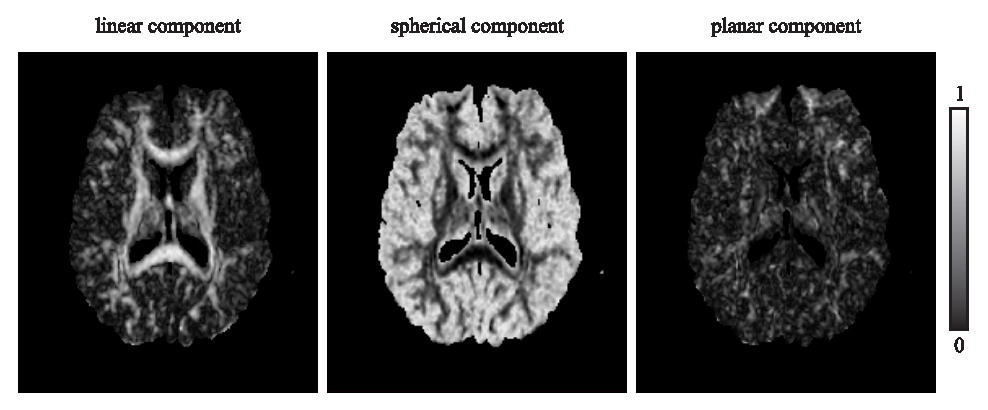
\includegraphics [scale=0.9,center] {DTI_quantMaps_spher.eps}
    \caption{\textbf{Componentes geométricos del tensor de difusión.} El tensor de difusión se visualiza como sus componentes esférico, lineal y plano, cuya suma es unidad.}
    \label{F:DTI_quantMaps_spher}
\end{figure}

En el algoritmo de asignación de fibra por seguimiento continuo (``FACT'') \citep{Mori_1999} (Figura 2.15), todos los voxels en el conjunto de datos que muestran un valor de FA por encima de un cierto umbral (típicamente en el intervalo de 0.25 a 0.30) son ``sembrados'' y cada línea se propaga según $\nu_1$. Cada vez que la línea se encuentra con el límite entre dos voxels, pregunta la dirección de $\nu_1$ y FA del voxel que está apuntando hacia. Si el valor de FA está por debajo de un umbral de alto (similar al umbral de inicio), o si el ángulo en el que se gira es grande y biológicamente implausible (por ejemplo,$>70$\textdegree{}) la línea de corriente se trunca. El algoritmo se ejecuta una segunda vez, ya que $\nu_1$ es bidireccional. Decidir la dirección del tracto en las intersecciones del voxel a diferencia de cada paso de longitud fija (que requiere la interpolación del tensor) aumenta la eficacia computacional. La selección de los umbrales de anisotropía y curvatura es dependiente del usuario y suele adaptarse a la meta en cuestión (es decir, los tramos de interés). Si se fija el umbral de FA demasiado alto, se minimiza la posibilidad de una propagación errónea a expensas de obtener menos tractos y dificultar la disección. Por el contrario, un umbral de FA muy bajo (por ejemplo $<0.10$) forzará al algoritmo a iniciar la propagación en áreas donde la dirección de difusividad principal podría ser biológicamente sin sentido o determinada por contribuciones de ruido (por ejemplo, en FCE). La misma idea se aplica al umbral de FA de terminación \citep{Mori_2002,Dauguet_2007}. El umbral de curvatura se hace a menudo muy estricto cuando se analizan tractos con curvatura mínima, como el tracto cortico-espinal. Para el análisis de las fibras U cortico-corticales, el umbral debe ser relajado, ya que estas conexiones se doblan bruscamente dentro de la sustancia blanca subcortical.

El algoritmo ``FACT'' tiene un buen rendimiento en los tramos curvos y la velocidad computacional en comparación con otros algoritmos \citep{Lazar_2003} (el cálculo del campo tensor y la generación de los tramos de fibra en un conjunto completo de datos de cobertura total del cerebro se realiza en menos de dos minutos). DTI-studio \citep{Jiang_2006}, es un software utilizado para realizar la tractografía, y se obtiene directamente de los Dres. Susumu Mori y Hangyi Jiang (Universidad Johns Hopkins). Este software tiene la ventaja de tener poderosas herramientas para disección virtual de los tractos (ver más abajo).

\begin{figure}
	\centering
    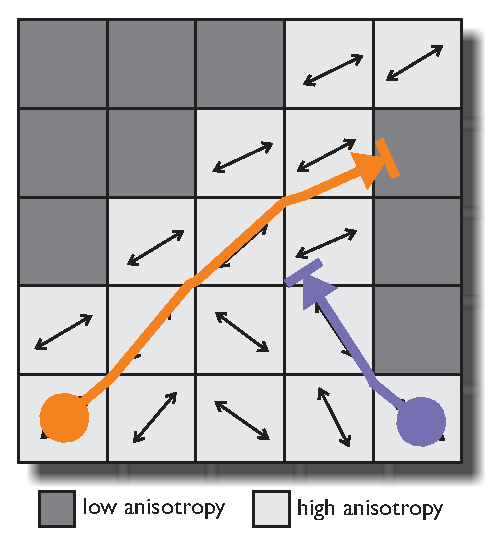
\includegraphics [scale=1,center] {DTI_FACT.eps}
    \caption{\textbf{Fibra de asignación por seguimiento continuo.} Todos los voxels en el conjunto de datos con anisotropía de alta difusión son ``sembrados''. En este ejemplo bidimensional simplificado, se muestran dos de los tramos resultantes. Las líneas se propagan en la misma dirección que la principal difusividad del voxel (flechas bidireccionales negras), cambiando su rumbo cada vez que encuentran un límite. El tracto naranja se detuvo cuando alcanzó un voxel con anisotropía baja, mientras que el tracto azul se detuvo cuando intentó hacer un giro brusco.}
    \label{F:DTI_FACT}
\end{figure}

Todos los algoritmos de propagación de líneas se pueden iniciar desde regiones de semillas específicas (determinadas por el usuario) o sembrando todo el cerebro. El problema con el primer enfoque es que sólo se puede obtener el mismo número de trazos que el número de semillas, limitando el número de tramas que intersectan el área de interés. Con el segundo enfoque, se obtienen miles de trazos, entonces el usuario selecciona sólo aquellos que pasan por una región específica, proporcionando generalmente mejores resultados, particularmente en áreas de ``ramificación'' de los haces \citep{Conturo_1999}. Con la siembra de todo el volumen, por lo tanto, es absolutamente necesario realizar la disección virtual de los haces de interés, sobre la base de un conocimiento {\it a priori} de su curso. La disección se realiza utilizando operadores booleanos, excluyendo todos los trazos resultantes que no cumplen con los criterios deseados. Dado que la mayoría de los haces de materia blanca tienen una trayectoria única que no es compartida por los fascículos circundantes, el investigador puede fácilmente proporcionar hitos a través de los cuales los trazos deben intersecarse (Figuras 2.16 y 2.17). La mayoría de los tractos requieren al menos dos regiones de selección de tracto para ser diseccionadas con éxito. Se han publicado pautas para la disección virtual de algunos tractos \citep{Catani_2002,Wakana_2007}, aunque a veces es necesario realizar algunos ajustes adicionales para su representación precisa, debido a diferencias en la calidad de imagen, adquisición, etc.

\begin{figure}
	\centering
    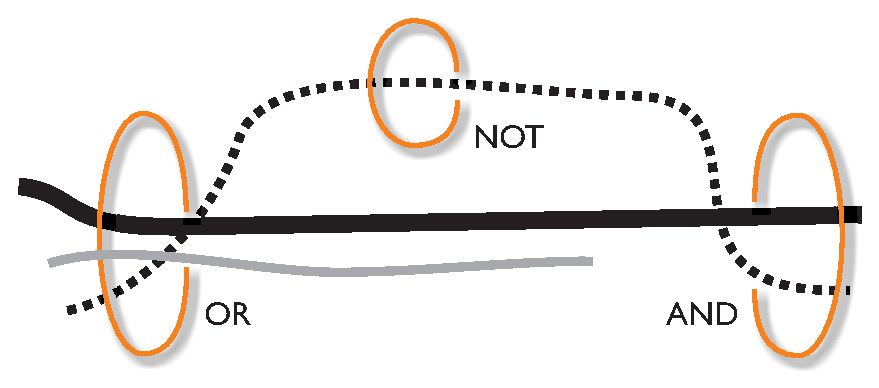
\includegraphics [scale=0.8,center] {DTI_dissection.eps}
    \caption{\textbf{Dissección virtual en tractografía.} Después de sembrar todos los voxels en el volumen con anisotropía alta, sólo se conservan los tramos de interés para su visualización y análisis posterior. Esto se logra colocando estratégicamente áreas a través de las cuales el tramo de interés debe pasar. El operador OR selecciona todos los trazos que pasan por la región. Sin embargo, el delgado tracto gris no pasa a través del operador AND y se desecha. Finalmente, el tramo de puntos, que muestra un camino extraño, se descarta utilizando un operador NOT.}
    \label{F:DTI_dissection}
\end{figure}

Una consideración importante de los algoritmos de propagación de línea es que los errores se acumulan a medida que se propagan las líneas. Es decir, para cada voxel hay una contribución de cierto ruido a la estimación del tensor y, a medida que las líneas se propagan y visitan consecutivamente más voxels, aumenta la probabilidad de que el tracto muestre una desviación aleatoria. La cantidad de incertidumbre en la orientación del tensor se puede calcular y visualizar utilizando el procedimiento bootstrap \citep{Jones_2003}. Sin embargo, para ello, es necesario obtener las imágenes individuales para cada dirección de gradiente antes del promedio. También se pueden emplear protocolos ITD que utilicen un promedio de imagen en línea, aumentando de este modo la relación señal-ruido y reduciendo el número total de imágenes en cada conjunto de datos a uno por segmento por dirección de difusión; por lo tanto, la estimación de la incertidumbre de orientación mediante el método ``bootstrap'' se excluye. No obstante, se puede utilizar favorablemente la acumulación de errores, ya que los trazos con trayectos incorrectos (determinados por la contribución de ruido) son claramente visibles y pueden eliminarse fácilmente utilizando el operador no booleano.

\begin{figure}
	\centering
    \includegraphics [scale=0.8,center] {DTI_CSTdissection.eps}
    \caption{\textbf{Disección virtual del tracto cortico-espinal.} Todos los voxels de anisotropía alta en los conjuntos de datos son sembrados, resultando en más de 200.000 tractos, 30\% de los cuales se visualizan en el panel a. Con el fin de prácticamente diseccionar este tramo particular de interés, los tractos deben pasar por tres regiones (basadas en un conocimiento anatómico a priori de la trayectoria del haz) identificadas en el panel d. El tracto resultante (byc), se colorea de acuerdo con la anisotropía. En los paneles b-d, la difusividad principal se denotan con componentes rojos, verdes y azules, superpuestos en imágenes de alta resolución T1 para una mejor apreciación del detalle anatómico.}
    \label{F:DTI_CSTdissection}
\end{figure}

Hay otro enfoque de la tractografía que no da lugar a trazos sintéticos que representan la vía de máxima verosimilitud, sino a la probabilidad de que exista una cierta conexión residente en cada voxel, apropiadamente denominada tractografía {\it probabilística} \citep{Behrens_2003}. Las principales ventajas del método son que caracteriza inherentemente la incertidumbre del modelo tensor, puede utilizarse en áreas de baja anisotropía (como la corteza y la materia gris subcortical) y es robusta al ruido. La tractografía probabilística se ha utilizado para segmentar con éxito los núcleos del tálamo, basándose en sus proyecciones a la corteza \citep{Behrens_2003}. La desventaja de este método de tractografía es que encuentra todas las áreas posibles del cerebro con una probabilidad no nula de conectarse a una región de ``semilla'', que a menudo incluye más de un haz de materia blanca. Por lo tanto, si el objetivo es identificar fascículos individuales, se prefieren los métodos determinísticos de propagación de líneas.

\section{Métodos para el análisis cuantitativo del\\ tensor de difusión}

Como se discutió anteriormente, el tensor de difusión y sus medidas derivadas se pueden visualizar como mapas, lo que permite el examen visual de parámetros de difusión cuantitativos. Además, existen métodos para extraer estos parámetros de mapas previamente calculados en uno o varios temas.

\textbf {Regiones de interés} El análisis de las regiones de interés (ROI) es quizás el más fácil de entender y realizar. En este enfoque, un contorno de dos (o tres) dimensiones se dibuja manualmente alrededor de la estructura de interés. Alternativamente, se puede colocar una forma geométrica de tamaño fijo (por ejemplo, una caja o una esfera) dentro de la estructura de interés. Los voxels incluidos en la región son consultados para los parámetros deseados y sus valores se promedian con el fin de proporcionar una sola medición por ROI. Dado que todos los mapas de difusión cuantitativos del mismo sujeto están espacialmente alineados, el mismo ROI puede operar en cada uno de los mapas de forma independiente. Es decir, para una estructura particular en un solo sujeto, el operador necesita esbozar la estructura de interés sólo una vez, y obtener los valores de ADC, autovalores, FA, etc. La medición directa de los mapas de difusión cuantitativa proporciona un enfoque directo para la prueba de hipótesis hechas {\it a priori}. El inconveniente es que los ROIs se colocan manualmente, lo que hace que este un procedimiento de tiempo y dependiente del usuario.

\textbf{Análisis basado en tracto} El tramo de interés se representa utilizando la tractografía en cada sujeto, y todos los voxels que contribuyen al tracto se tratan como un ROI tridimensional. Este enfoque tiene la ventaja de utilizar la naturaleza semi-automatizada de la tractografía, donde las regiones de selección de trazado pueden definirse de forma poco definida (Figura 2.17), minimizando la dependencia del método por parte del usuario. Es decir, el usuario no tiene que bosquejar con precisión una estructura de interés, sino simplemente proporcionar una (o más) áreas amplias a través de las cuales un tramo debe pasar y aprovechar los operadores booleanos (Figura 2.16) y el conocimiento anatómico del trayectoria del tracto. Más importante aún, ciertas estructuras con una delgada sección transversal y/o curvas caminos se representan más fácilmente utilizando tractografía que con varios ROIs. Al igual que con los ROI, el investigador debe elegir las estructuras que se analizarán con antelación.

\textbf{Mapeo paramétrico estadístico} El análisis de cada estructura sobre cada sujeto puede ser un proceso engorroso y largo si el tamaño de la muestra es grande. Esencialmente, en la cartografía paramétrica estadística (SPM) los volúmenes cerebrales de los sujetos incluidos en el estudio son ``morphed'' y se hacen para que coincida con una plantilla (o atlas) tan cerca como sea posible, después de lo cual las estadísticas se realizan en un pixel por pixel base. A continuación se destacan diferencias significativas en la plantilla, mostrando las regiones del cerebro que difieren entre los grupos estudiados. Este método fue tomado de la morfometría basada en voxel de los volúmenes cerebrales \citep{Wright_1995,Ashburner_2001} y, aunque es muy atractivo, sufre de varios problemas, el mayor de los cuales es el hecho de que la transformación de la imagen (normalización) de volúmenes individuales a la plantilla nunca es Perfecto. En particular, mientras que la forma general, el tamaño y la posición de dos cerebros diferentes pueden ser adecuadamente emparejados, las diferencias individuales sutiles de las estructuras intraparenquimatosas no pueden \citep{Ashburner_2001}. Con el fin de superar este problema (y para satisfacer los requisitos estadísticos del método), las imágenes normalizadas son generalmente borrosa utilizando un núcleo gaussiano. Aunque técnicamente es un método analítico independiente del usuario, en realidad el usuario debe seleccionar varios parámetros diferentes, como el ancho del núcleo gaussiano borroso, que puede influir en gran medida en los resultados y las conclusiones derivadas de ellos \citep{Jones_2005,Jones_2007}. Su mayor ventaja (una desventaja en manos inexpertas) es el hecho de que el investigador no necesita tener una hipótesis {\it a priori}, lo cual es útil en condiciones donde no se conoce la ubicación de las sospechas de anomalías.

\textbf{Estadísticas espaciales basadas en el tracto} Este es un nuevo enfoque presentado recientemente por Smith {\it et al}. \citep{Smith_2006}, que minimiza los problemas de SPM y permite que las comparaciones de cerebro completo se realicen sin hipótesis {\it a priori}. En este método, los mapas FA están alineados con una plantilla, y de la media de todos los mapas FA se obtiene un ``esqueleto'' de los tractos de materia blanca. Luego, se crea un mapa de esqueleto para cada sujeto proyectando sus mapas de FA en el espacio estándar y rellenando el esqueleto con los valores de FA del centro del tramo más cercano. Esto intenta posicionar todos los sujetos en el mismo espacio, con cada voxel que representa exactamente la misma estructura de la materia blanca. Después de esto se logra, se pueden realizar estadísticas voxelwise a través de sujetos. Al igual que la SPM, se destacan las diferencias significativas, de las cuales la tractografía probabilística puede ser iniciada opcionalmente. La desventaja de este método es que sólo analiza una proporción relativamente pequeña de toda la sustancia blanca disponible, es decir, sólo aquellos voxeles con anisotropía alta. Se pierde información valiosa de un gran número de voxels en varias estructuras de materia blanca. Además, muchos tractos de materia blanca (por ejemplo, el tracto corticoespinal) están organizados somatotópicamente (es decir, tienen un orden anatómicamente definido dentro de ellos), haciendo que el análisis de su porción central sea un sesgo potencial.

\section{Deficiencias de DTI}
\subsection{El modelo}

El modelo de tensor de difusión puede identificar con precisión la arquitectura tisular en los casos en que hay homogeneidad de la estructura dentro del voxel muestreado. Sin embargo, no todas las áreas de la sustancia blanca muestran homogeneidad, particularmente en regiones donde dos o más poblaciones de fibras se cruzan entre sí. En estos casos, el modelo de tensor de difusión no puede identificar la orientación compleja del tejido. La razón detrás de este fracaso es que en DTI, se supone que existe un solo compartimiento de difusión gaussiana dentro de cada voxel. La adición de dos tensores prolatos (es decir, $\lambda_{1} > \lambda_{2,3}$) da como resultado un tensor oblato (es decir,$\lambda_{1} < \lambda_{2} = \lambda_{3}$) (Figura 2.18). Por lo tanto, el problema reside en el propio modelo, y la sobreestimación del tensor de difusión mediante la adquisición de imágenes con múltiples direcciones de gradiente de difusión no es útil.

Es común encontrar áreas de baja anisotropía profundamente dentro de la materia blanca del cerebro, que se podría considerar incorrectamente las lesiones. Por ejemplo, la región donde el fascículo longitudinal superior (orientación antero-posterior) cruza la corona radiata (superior-inferior) y el cuerpo calloso (izquierda-derecha) aparece como un ``agujero'' negro en los mapas FA. Además, dado que la mayoría de los algoritmos de tractografía de propagación de línea se detienen cuando alcanzan un área de baja anisotropía, estos trazos son truncados típicamente en este punto. La tractografía probabilística, que no está limitada por regiones de baja anisotropía donde la orientación es incierta, avanzará en muchas direcciones. La incertidumbre en estas áreas se representará por voxels más lejos a lo largo de la ruta de menor probabilidades asociados con ellos \citep{Behrens_2003}.

\begin{figure}
	\centering
    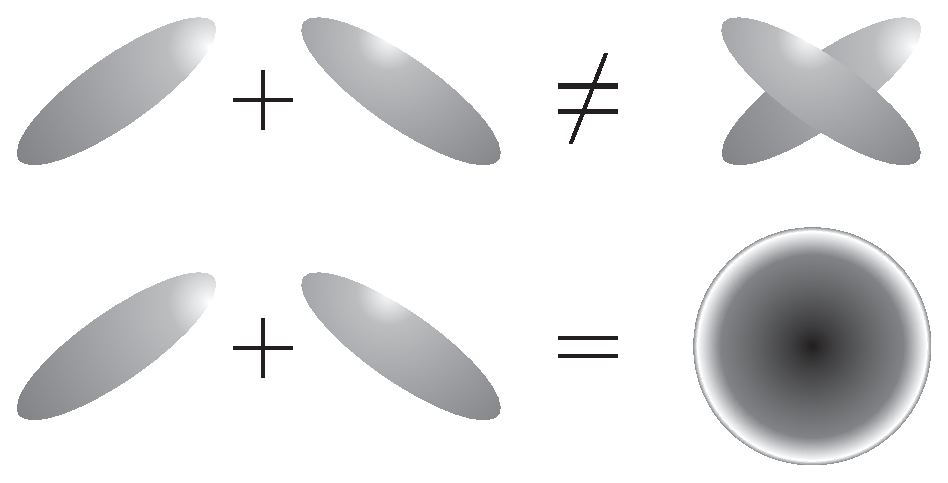
\includegraphics [scale=0.7,center] {DTI_tensorAddition.eps}
    \caption{\textbf{Adición de tensores de difusión.} Cuando dos poblaciones de fibras con diferentes orientaciones ocupan el mismo espacio, el modelo tensor no puede diferenciar las dos orientaciones, ya que la adición de dos tensores de difusión prolatos orientados perpendicularmente da lugar a un elipsoide oblato.}
    \label{F:DTI_tensorAddition}
\end{figure}

La verdadera función de difusión en las zonas de cruce de fibras es compleja. Por esta razón, las descripciones libres de modelo del perfil de difusión han sido desarrolladas \citep{Alexander_2002,Tuch_2004}, comúnmente denominadas imágenes de espacio Q o imágenes de difusión de alta resolución angular. En resumen, la función de difusión está relacionada con la señal de RM por la transformada de Fourier con respecto al vector de onda de difusión experimental {\it q} (el gradiente de difusión y su dirección) \citep{Stejskal_1965, Tuch_2004}. Los métodos de espacio Q utilizan alta resolución angular a altos valores de {\it b} y un gran número de direcciones de gradiente de difusión (generalmente más de 100). La sensibilidad de difusión ({\it b}) se incrementa para aumentar el contraste entre el componente de difusión rápida de las dos (o más) poblaciones de fibras \citep{Tuch_2003}. El objetivo es muestrear con precisión el perfil de difusión en cada voxel. En el caso de una sola población de fibra, el perfil de difusión se asemeja a un cacahuete (la difusión es mayor sólo en el eje principal del cacahuete), mientras que en el caso de dos o más poblaciones el cacahuete se convierte en una estructura multi-lobulada simétrica similar a una flor. En particular, los picos del perfil de difusión no corresponden a las direcciones de las fibras. Con el fin de obtener estos, se utiliza  la transformación de Funk-Radon \citep{Tuch_2004}. Una vez que se ha encontrado la orientación de las fibras, los algoritmos de tractografía modificada pueden representar haces de materia blanca, incluso en áreas donde se intersectan. Aunque estas mediciones de difusión libres de modelos son muy útiles, no han recibido tanta atención como lo ha hecho ITD, tal vez debido a los tiempos de adquisición muy largos requeridos, la gran cantidad de datos necesarios para recrear el perfil de difusión y, lo más importante, que las medidas escalares ITD se interpretan más fácilmente desde un punto de vista biológico. En esta disertación no se realizaron análisis de difusión de alta angular, sin modelo, ya que los correlatos biológicos de ITD son más conocidos que los de estos nuevos métodos.

Tanto la ITD como la Q-ball comparten un inconveniente, que es su incapacidad para discernir aferentes de las fibras eferentes. Es decir, mientras que la conectividad entre dos áreas puede inferirse y visualizarse, su direccionalidad sigue siendo desconocida.

\subsection{Artefactos de imagen}

Típicamente, los experimentos ITD in vivo humanos usan volúmenes de voxel que varían de 6 a $20 mm^{3}$. Dada esta restricción, sólo los haces de materia blanca con dimensiones considerablemente mayores que el tamaño del voxel pueden ser identificados y caracterizados correctamente. Por lo tanto, se pueden representar adecuadamente estructuras grandes, como el cuerpo calloso, las cápsulas internas o el fórnix, pero varias conexiones pequeñas pero importantes no pueden identificarse de forma fiable con ITD.

Es importante recordar que la información de los tensores disponibles en cada voxel corresponde al promedio ponderado de todas las clases de tejidos que residen en el mismo. Por lo tanto, si un voxel particular está ocupado por FCE y MB altamente coherente, el tensor resultante no será altamente anisotrópico, sino algo isotrópico (es incluso probable que tenderá más hacia el caso isotrópico, dada la difusión muy rápida de FCE y la señal alta obtenida de ella con ITD convencional - el TE largo utilizado favorece las especies T2 largas). De hecho, el {\it promedio de volumen parcial}, como se conoce como este artefacto, puede reducirse aumentando la resolución de las imágenes (reduciendo efectivamente el tamaño del voxel, minimizando la posibilidad de tener más de un tipo de tejido por voxel). Un aumento en la resolución tiene un alto precio, ya que está inversamente relacionado con la relación señal-ruido con tiempos de adquisición fijos. La mayor fuente de preocupante volumen parcial de promediado en el DTI es la contaminación de la señal con LCR, particularmente en aquellos paquetes de MB en proximidad cercana al LCR \citep{Concha_2005}. Afortunadamente, prácticamente toda la señal procedente del FCE puede ser anulada específicamente, limitando su contribución al tensor resultante en voxels con volumen parcial. Esta técnica se basa en las diferencias en la relajación longitudinal del LCR y del tejido cerebral. Brevemente, se aplica un impulso de inversión antes de la excitación de la muestra, en un tiempo calculado a partir de la constante T1 de FCE. La muestra se excita entonces precisamente cuando la magnetización longitudinal del LCR pasa por cero, pero la de otros tejidos es finita.

La resolución de las técnicas actuales de ITD está restringida por la secuencia de generación de imágenes usada para adquirir los datos, que a su vez está restringida por el hardware (particularmente la resistencia a gradientes). El IPD se utiliza generalmente, ya que permite imágenes muy rápidas, lo cual es absolutamente necesario dado el gran número de imágenes necesarias para construir un volumen de ITD (por ejemplo, con seis direcciones de gradiente de difusión, una imagen ponderada de no difusión por rebanada, ocho promedios y 60 rebanadas: $7×8×60 = 3360$ imágenes) y para minimizar los artefactos de movimiento. El tiempo de adquisición corto alcanzado con IPD se logra utilizando un solo impulso de radiofrecuencia de excitación de spin (es decir, un solo impulso de 90\textdegree{}), después de lo cual se llena la totalidad del espacio {\it k} alternando entre gradientes de codificación de frecuencia positiva y negativa precedido por blips del gradiente de codificación de fase (Figura 2.19). El movimiento del paciente se minimiza así, ya que cada imagen es esencialmente una "instantánea" de la posición actual.

\begin{figure}
	\centering
    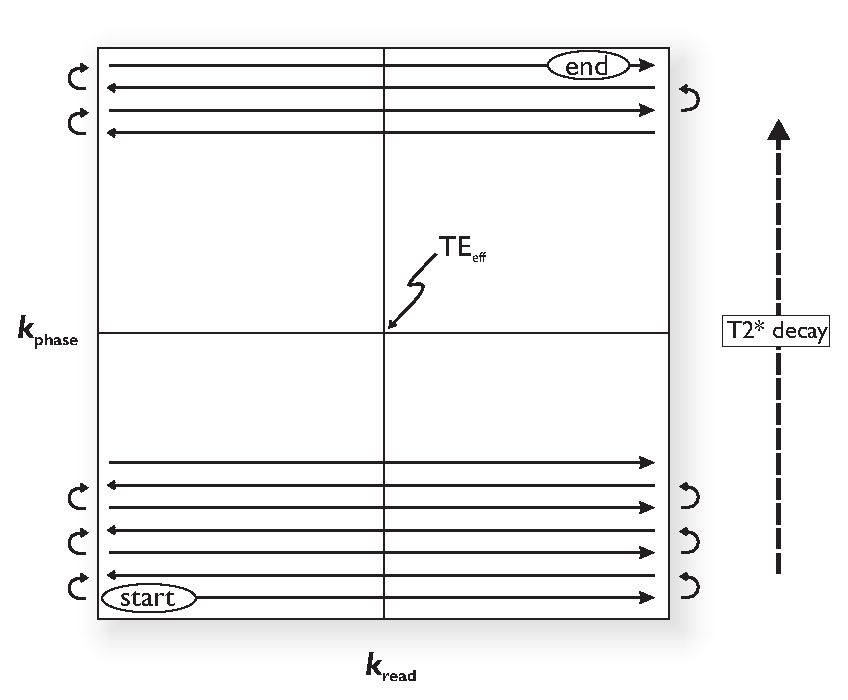
\includegraphics [scale=0.7,center] {kspace.eps}
    \caption{\textbf{Trayectoria de adquisición de IPD en {\it k}-espacio (dominio de frecuencia).} Después de una sola excitación, se adquieren líneas alternas de espacio {\it k}, precedidas por "blips" de los gradientes de codificación de fase. El TE efectivo (TE e f f) está determinado por la línea de adquisición que atraviesa el centro del espacio {\it k}. La señal disponible se desintegra según la constante T2 * del tejido a lo largo de la adquisición del espacio-k.}
    \label{F:kspace}
\end{figure}

Por desgracia, en la velocidad de IRM tiene un precio. Dos artefactos muy evidentes vistos en ITD son causados por la secuencia de IPD, ambos de los cuales son aún mayores en fuerzas de campo más altas. El primer artefacto IPD potencial se llama N/2 o fantasma Nyquist. Las inconsistencias de los ecos pares e impares causan desplazamientos de fase que producen un fantasma desplazado por la mitad de los píxeles de campo de visión (FOV) en la dirección de codificación de fase, en relación con la imagen real. Si el FOV es lo suficientemente grande, estos fantasmas aparecen fuera de la imagen real y no son intrusivos. Sin embargo, esto no siempre es el caso, para lo cual se han propuesto varios métodos de corrección que adquieren datos de referencia adicionales \citep{Hu_1996,kuei_2004} o utilizan esquemas de posprocesamiento \citep{kuei_2004,Zhang_2004}. El segundo artefacto del IPD se debe a inhomogeneidades de campo magnético que alteran la fase de los giros, con una posterior interpretación errónea de su ubicación en el espacio. La diferencia de susceptibilidad magnética se hace más evidente por la decadencia de señal de T2* que se produce durante la lectura de IPD en la dirección de codificación de fase (Figura 2.19). {\it Distorsiones geométricas}, como este segundo artefacto se conoce como, son más aparentes cerca de las interfaces de tejido, sobre todo si poseen susceptibilidades magnéticas muy diferentes, como el aire y el tejido. Por lo tanto, este artefacto es evidente cerca de los senos para-nasales o en la base del cráneo, donde parece que el cerebro ha sido ``aplastado'' (para la codificación de la fase anterior-posterior) o cortado (en la izquierda-derecha de codificación de fase). Al igual que con los artefactos N/2, se han publicado varios métodos que intentan minimizar los artefactos no resonantes \citep{Weiskopf_2005,Jezzard_1995,Reber_1998}. Los tiempos de adquisición largos pueden reducirse concatenando la adquisición de espacio {\it k} usando dos o más lecturas de IPD (a expensas de al menos duplicar el tiempo total de adquisición de imagen) \citep{99,100}; o reduciendo el número de líneas de espacio {\it k} adquiridas a través de Fourier de fase parcial o imágenes paralelas \citep{Pruessmann_1999}.

Aunque es cierto que el movimiento se minimiza en cada una de las adquisiciones de IPD, tengo que hacer dos notas especiales. En primer lugar, el movimiento puede ocurrir entre adquisiciones sucesivas, produciendo un desajuste dentro de diferentes direcciones de gradiente de difusión, haciendo que el cálculo de ADC carezca de sentido (recuerde que ADC se calcula en una forma de pixel por pixel). En segundo lugar, artefactos de movimiento sutiles, involuntarios pueden surgir debido a fenómenos fisiológicos, tales como las pulsaciones de baja amplitud del cerebro y FCE \citep{107}. Este movimiento sutil conduce potencialmente a estimaciones artifactually altas de ADC 108. Se ha informado de que la adquisición de las imágenes basadas en el ciclo cardíaco (es decir, la activación cardiaca o la activación / activación del pulso) minimiza los artefactos de pulsación \citep{108,109}. En este enfoque, cada imagen se adquiere precisamente al mismo tiempo con respecto a la onda de pulsación (por ejemplo, 500 ms después de la onda R). Esto se produce a expensas de aumentar el tiempo de escaneo \citep{108}. El uso de la supresión del LCR \citep{Concha_2005} complica el uso de la activación cardiaca / del pulso, pero también disminuye los efectos de los artefactos de pulsación, razones por las cuales no realizamos ninguna forma de activación en los estudios discutidos en la presente memoria.

La segunda fuente de artefactos en IPD y ITD son los propios gradientes de difusión. Los gradientes alternantes rápidos producen corrientes parásitas adicionales que afectan negativamente al campo magnético principal. Los campos magnéticos residuales causados por las corrientes parásitas producen traducciones de imágenes y distorsiones geométricas. La secuencia DTI utilizada a lo largo de esta tesis se basa en una secuencia de IPD de un solo disparo, dos veces enfocada, \citep{110} (Figura 2.20). Esta secuencia es una modificación de la secuencia de spin-eco de Stejskal y Tanner (Figura 2.3) que separa el par de gradientes de difusión-codificación en dos pares (cada par con su respectivo pulso de reorientación). La descomposición de los gradientes de difusión minimiza las corrientes parásitas antes de la lectura IPD, produciendo menos distorsiones geométricas y traducciones de imágenes. Esto es de particular importancia puesto que las imágenes IPD deben espaciar espacialmente la imagen no ponderada por difusión para calcular adecuadamente el ADC en cada píxel. Sin embargo, como la lectura se basa en IPD, las imágenes todavía sufren de ligeras distorsiones geométricas en la dirección antero-posterior (la dirección de codificación de fase); afortunadamente, estas distorsiones están muy lejos de los haces de interés de la materia blanca (ver por ejemplo los lóbulos frontales en la Figura 2.9, panel a).

Otro efecto de la lectura larga de IPD es la susceptibilidad a efectos de cambio químico. En particular, la grasa y el agua tienen diferentes frecuencias de resonancia (separadas por 3,3 partes por millón, 210 Hz a 1,5T), lo que da como resultado un fantasma de imagen derivado de grasa que se desplaza espacialmente (en la dirección de codificación de fase) imagen derivada. Este problema se supera fácilmente mediante la utilización de la supresión espectral de grasa antes de la excitación. En este enfoque, los tejidos grasos se excitan selectivamente utilizando un pulso de radiofrecuencia en resonancia con la velocidad precesional de los protones grasos, después de lo cual la magnetización transversal residual se descompone (``estropeada'') con un pulso de gradiente (figura 2.20). La excitación de las moléculas de agua sigue inmediatamente, y la señal resultante está desprovista de contribuciones de grasa.

La secuencia ITD utilizada en esta disertación tenía ligeras distorsiones geométricas en la parte más anterior de los lóbulos frontales y cerca de la base del cráneo que no fueron compensados por el enfoque dos veces reorientado. Sin embargo, estos artefactos se encuentran distantes de las áreas de interés y no afectan las mediciones realizadas. Incluso el hipocampo está lo suficientemente lejos del hueso petroso para escapar de este artefacto. Se utilizó un esquema de codificación de frecuencia izquierda-derecha y, por lo tanto, se producen distorsiones geométricas en la dirección antero-posterior (causando, por ejemplo, que los polos frontales aparezcan comprimidos). N/2 artefactos fueron mínimos y no intrusivo en las imágenes adquiridas, ocupando principalmente el espacio vacío en la imagen debido a la amplia FOV empleado.

\begin{figure}
	\centering
    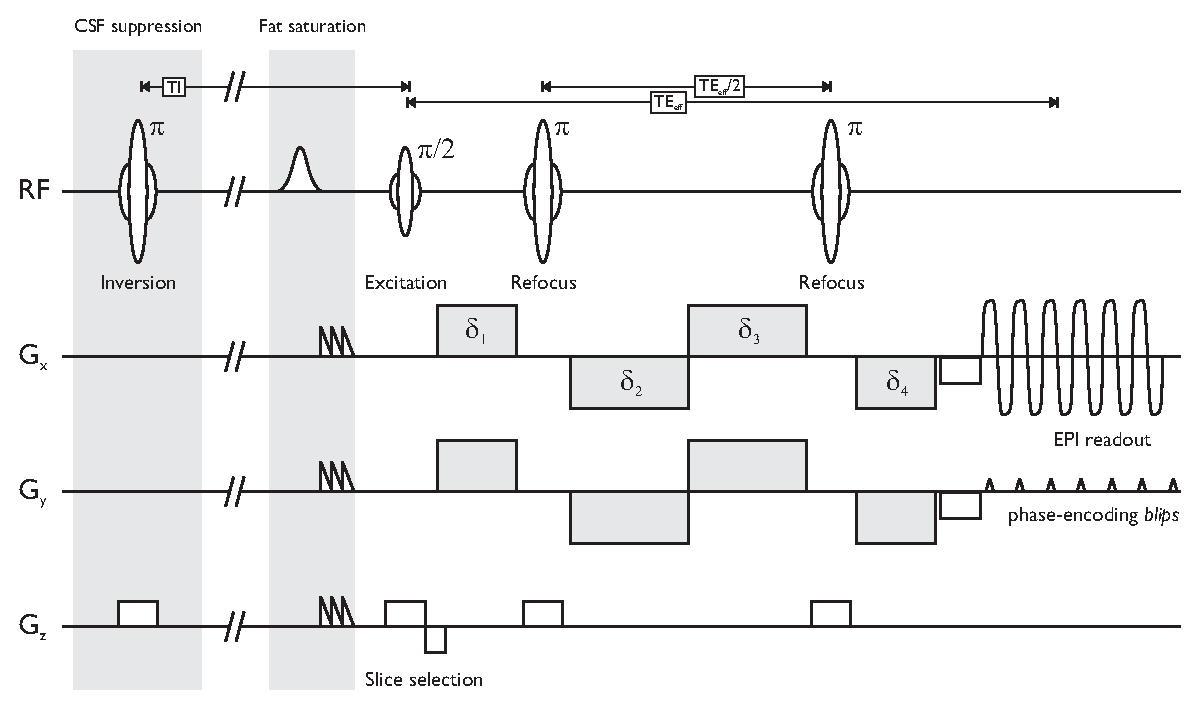
\includegraphics [scale=0.7,center] {ReeseDTI.eps}
    \caption{\textbf{Diagrama de secuencia de DTI basado en IPD, doblemente reenfocado, suprimido en LCR.} Un impulso de inversión selectiva se aplica antes del impulso de excitación, separado por un tiempo de inversión (TI) de alrededor de 2200 ms. Esto suprime selectivamente la señal de FCE, basada en su T1 largo. La supresión espectral de grasa se utiliza antes de la excitación. Se utiliza un conjunto de cuatro gradientes alternantes de sensibilización a la difusión, que compensan sus corrientes inducidas inducidas, minimizando distorsiones de imagen. Un tren de lectura IPD codifica la información espacial. En este ejemplo particular, los gradientes de difusión se han aplicado en las direcciones x (lectura) e y (fase).}
    \label{F:ReeseDTI}
\end{figure}

Dadas las limitaciones de la técnica IPD, se han desarrollado alternativas para la adquisición de imágenes ponderadas por difusión \citep{111-116}. Sin embargo, estos nuevos métodos están lejos de ser tan ampliamente disponibles como un solo disparo IPD basado ITD. Además, requieren el uso de varios impulsos de excitación (es decir, no son ``de disparo único''). Estos impulsos de excitación extra aumentan el tiempo necesario para adquirir la imagen, aumentando la susceptibilidad al movimiento del sujeto y el tiempo de exploración total. Además, dada la gran cantidad de imágenes adquiridas durante una sesión típica de DTI, la potencia extra de radiofrecuencia depositada sobre el sujeto podría alcanzar niveles inaceptables y causar calentamiento. A pesar de la presencia de los artefactos de formación de imágenes mencionados anteriormente inherentes a la misma, IPD proporciona todavía un equilibrio apropiado entre la velocidad de adquisición, la calidad de imagen y la deposición de radio-frecuencia.

Cabe señalar nuevamente que incluso si las imágenes de muy alta resolución pudieran ser adquiridas con calidad adecuada y carentes de todos los artefactos de imagen, la capacidad del ITD para diferenciar entre dos o más poblaciones de fibras se limita al propio modelo tensor. Finalmente, si bien los mecanismos biofísicos de anisotropía de difusión han sido estudiados en modelos animales \citep{Beaulieu2002}, todavía no se sabe si los mismos mecanismos subyacen a la anisotropía de difusión observada en la sustancia blanca humana. Como tal, la inferencia de la integridad del tejido a través del análisis del tensor de difusión requiere suposiciones importantes que no han sido completamente validados en los seres humanos. La base de la anisotropía en tejido humano se estudia con más detalle en las referencias \citep{Beaulieu2002,117,118}.

\section{Cuando el modelo del tensor no es suficiente\footnote{Esta sección se toma del trabajo del autor publicado en otra parte \citep{118}}}

Con el reconocimiento de que el uso de la resolución típica casi el 90\% de los voxels de la sustancia blanca en el cerebro humano contienen fibras cruzadas \citep{119} y que el modelo tensor es inadecuado en estas circunstancias (véase la figura 2.18), existe una necesidad definida de encontrar formas alternativas de analizar la señal de difusión MRI que transmiten información sobre microestructura de tejidos complejos. Hay varios métodos para tratar este problema \citep{120}, pero todos tienen una cosa en común, y ése es su alta demanda en términos de adquisición de datos en comparación con DTI. Algunos métodos de espacio q requieren varias decenas de direcciones de gradiente de difusión con uno o más valores b altos ($2.000-50.000 s/mm^{2}$), lo que potencialmente se traduce en tiempos de adquisición prohibitivamente largos ($> 25$ min). Afortunadamente, los recientes desarrollos en hardware, diseño de secuencias de pulso y métodos analíticos \citep{Tuch_2002,121} están reduciendo progresivamente el tiempo de escaneo y las alternativas al DTI se están haciendo factibles en el ámbito clínico \citep{122}. Las ventajas de los enfoques no tensionales de la tractografía son evidentes e indiscutibles \citep{123}, ya menudo es absolutamente necesario poder resolver las fibras cruzadas para identificar ciertos haces de materia blanca, como la radiación acústica o los aspectos laterales de la tractografía los tramos córtico-espinales \citep{124}. En el nivel de voxel único es posible obtener métricas de anisotropía de difusión similares a FA, aunque su interpretación biológica no ha sido tan bien estudiada como su contraparte tensor. Por ejemplo, el índice 87 de anisotropía fraccionaria generalizada (GFA), definido como la desviación estándar dividida por el cuadrado medio de la función de densidad de orientación de difusión, proporciona un reemplazo directo de FA en datos no tensoriales. Por diseño captura la anisotropía de todas las poblaciones de fibra a la vez y, por lo tanto, es incapaz de liberar las anomalías de los tejidos en poblaciones de fibra separadas. La construcción de toda la función de densidad de probabilidad de difusión (PDF) a través de uno de los métodos de espacio q [por ejemplo, imagen de espectro de difusión \citep{125} o imagen de bola q \citep{Tuch_2004} permite la extracción de parámetros que pueden ser alterados por 126 usos de alto valor b datos para estudiar el comportamiento y la orientación de la difusión del agua dentro y fuera de las neuritas (axones y dendritas), proporcionando así una descripción más completa de la organización de tejidos. En una preparación ex vivo de cerebro de roedor, la obtención de imágenes de espectro de restricción fue capaz de capturar importantes detalles estructurales de capas corticales que correspondían a histología pero no eran evidentes a través de otros métodos de difusión MRI. Los requerimientos de datos deben ser menos estrictos al imaginar el cerebro humano vivo, para el cual se han hecho adaptaciones de estos métodos analíticos. Por ejemplo, el diámetro axonal promedio y la densidad de grandes paquetes de materia blanca pueden determinarse dentro de los tiempos de adquisición aceptables (mientras que las simulaciones mostraron que el método funcionó bien y los resultados en seres humanos están en consonancia con las características histológicas conocidas, no hay evidencia directa de que el derivadas métricas axonales corresponden a histología). Además, se ha estimado la dispersión de neuritas y la densidad \citep{127} en humanos en menos de 30 minutos usando alta resolución angular y dos valores de cero no igual a cero. Como la anisotropía fraccional puede verse afectada de manera similar por el aumento de la dispersión de fibras o la reducción de la densidad de fibras, cada una con orígenes y significados muy diferentes, la capacidad de desambiguar las dos condiciones puede proporcionar información biológica importante y los tiempos de exploración relativamente cortos necesarios para adquirir todos los datos necesarios hacen que esta técnica sea atractiva para la investigación clínica.

Utilizando un único valor {\it b} no nulo y múltiples direcciones de gradiente, la función de distribución de orientación de fibras (fODF) puede obtenerse a través de la deconvolución esférica \citep{128}. La amplitud del FODF es proporcional a la fracción intra-axonal, así como al diámetro axonal y espaciamiento \citep{129,130}. Se han obtenido resultados convincentes por simulación de fibras, y la aplicabilidad de este método se ha demostrado en datos humanos, lo que demuestra que es más sensible que los parámetros DTI para identificar los cambios patológicos en la enfermedad de la motoneurona \citep{129}. Sin embargo, ningún estudio ha confirmado que los mecanismos sospechosos que impulsan los cambios en la amplitud del fODF corresponden verdaderamente a los cambios histológicos.

La difusión por resonancia magnética es una poderosa herramienta para la evaluación no invasiva de la microestructura de los tejidos; explora ingeniosamente la información relativa al comportamiento de la difusión del agua, empleándola para sondear el entorno microscópico mientras se informa a una escala macroscópica. Proporciona una ventana en el reino microscópico en cada vóxel de la imagen, mientras que al mismo tiempo que permite la identificación de macroscópica, de largo alcance las vías de la materia blanca a través de la tractografía. La relativa facilidad con que se puede aplicar para estudiar el cerebro humano lo ha hecho muy popular entre los científicos y los médicos, y la técnica está ahora disponible en prácticamente todos los escáneres modernos. Sin embargo, al igual que con cualquier herramienta poderosa, debemos ser conscientes de su alcance y sus limitaciones, teniendo en cuenta que cualquier inferencia sobre la microestructura de los tejidos surge de una medición indirecta y debe considerar todos los factores (biológicos y artefactuales) que pueden influir en la difusión antes de hacer declaraciones en negrita sobre la integridad de la materia blanca.
\clearpage
\bibliographystyle{unsrtnat} 
\bibliography{libroResonancia.bib}
    
\end{document}